%========================================================
% CHAPTER 3 — Numerical Simulations and Results
%========================================================

The fiber-channel models developed in the previous chapter are investigated
numerically in this chapter with the objective of determining how the physical
properties of the source and optical link affect the operational suitability of
the distributed polarization-entangled state.

The numerical analysis is organized around the mapping

\begin{equation}
\boxed{
\boldsymbol{\xi}
\longrightarrow
\boldsymbol{\lambda}(\boldsymbol{\xi}),
}
\label{eq:chapter3_physical_operational_mapping}
\end{equation}

where \(\boldsymbol{\xi}\) collects the relevant source, fiber, and compensation
parameters, while \(\boldsymbol{\lambda}\) contains the quantities used to
characterize the resulting two-photon polarization state. In the present
analysis, particular attention is given to purity, fidelity, concurrence, and
the basis-dependent quantum bit error rates \(Q_Z\) and \(Q_X\).

The central objective is to determine the combinations of physical parameters
for which the optical link remains compatible with the adopted BBM92
requirement. The numerical simulations therefore focus on the identification
and interpretation of the operating region

\begin{equation}
\boxed{
\mathcal{R}_{\mathrm{BBM92}}
=
\left\{
\boldsymbol{\xi}
:
Q(\boldsymbol{\xi})
<
Q_{\mathrm{th}}
\right\},
}
\label{eq:chapter3_bbm92_operating_region}
\end{equation}

where \(Q_{\mathrm{th}}\) denotes the QBER threshold associated with the security
assumptions adopted for the analysis.

The study follows the modeling hierarchy introduced in
Chapter~\ref{ch:02_fiber_channel_modeling}. Effective polarization-only models
are first used to isolate the relation between different degradation mechanisms,
state-quality metrics, and BBM92 errors. The analysis is then extended to
frequency-dependent birefringent propagation, allowing the operating region to
be expressed directly in terms of source and fiber parameters such as spectral
bandwidth, differential group delay, spectral correlation, and the relative
properties of the two propagation arms.

Particular attention is devoted to the distinction between state-quality and
operational quantities. Concurrence characterizes the surviving bipartite
entanglement, while purity and fidelity provide complementary information on the
propagated state. BBM92 operation, however, depends directly on the correlations
observed in the protocol measurement bases and is therefore assessed through the
corresponding QBER. The numerical analysis consequently investigates both the
relation and the differences between these descriptions.

The experiments progressively examine the effects of individual channel
mechanisms, source--fiber parameter combinations, two-arm propagation,
compensation errors, and modeling approximations. The final objective is to
construct operating maps that identify the physical configurations belonging to
\(\mathcal{R}_{\mathrm{BBM92}}\) and quantify how its boundary changes with the
properties and modeling of the optical link.


%========================================================
% SECTION 3.1 — Computational Framework
%========================================================

\section{Computational Framework and Numerical Methodology}
\label{sec:computational_framework_matlab}

All numerical models presented in this chapter are implemented in MATLAB using a
modular library that reproduces the mathematical structure introduced in the
theoretical framework. Quantum states, density operators, polarization
transformations, quantum channels, and measurement observables are represented
directly through complex vectors and matrices.

Reusable numerical routines provide the common operations required throughout
the analysis, including state preparation, local evolution, quantum-channel
application, frequency-dependent fiber propagation, spectral averaging,
polarization measurements, and state characterization. The numerical simulations
are constructed from these common components, ensuring that different physical
configurations and modeling assumptions are evaluated using the same underlying
computational framework.

For a specified physical configuration \(\boldsymbol{\xi}\), the numerical
workflow is summarized by

\begin{equation}
\boxed{
\boldsymbol{\xi}
\longrightarrow
\rho_{AB}(\boldsymbol{\xi})
\longrightarrow
\boldsymbol{\lambda}(\boldsymbol{\xi})
\longrightarrow
\mathcal{R}_{\mathrm{BBM92}}.
}
\label{eq:numerical_workflow_chapter3}
\end{equation}

For effective polarization channels, the propagated density operator is obtained
directly from the corresponding channel action. For frequency-dependent fiber
models, the two-photon state is propagated over the joint spectrum and the
unresolved spectral degree of freedom is subsequently traced out to obtain the
reduced polarization density operator.

The resulting state is characterized using a common set of quantities throughout
the numerical study. Purity, fidelity, and concurrence describe complementary
properties of the distributed quantum state, while the polarization measurement
statistics determine \(Q_Z\) and \(Q_X\). The latter provide the direct criterion
used to classify each simulated physical configuration with respect to the
adopted BBM92 operating condition.

The numerical simulations presented below therefore use the simulator primarily
as a parameter-space analysis tool. Rather than considering isolated propagation
examples, each experiment is designed to determine how a specific physical
mechanism or modeling assumption modifies the boundary between operational and
non-operational regions of the optical link.


%========================================================
% SECTION 3.2 — Experiment 1
%========================================================

\section{Effective Fiber Models and BBM92 Performance}
\label{sec:effective_models_bbm92_performance}

%========================================================
% Experiment 1 — Effective Fiber Models and BBM92 Performance
%========================================================

\subsection{Objective and Numerical Setup}

The first numerical experiment compares the effective fiber models introduced in
Chapter~\ref{ch:02_fiber_channel_modeling} from both a state-characterization
and an operational BBM92 perspective. The objective is to distinguish changes in
the quality of the distributed entangled state from changes in the correlations
observed in the fixed protocol measurement bases.

The input state is \(|\Psi+\rangle\) and three mechanisms are considered: coherent relative-phase evolution, statistical
dephasing, and symmetric local depolarization. For each propagated state, the
purity \(\gamma\), fidelity \(F\), concurrence \(C\), and basis-dependent error
rates \(Q_Z\) and \(Q_X\) are evaluated.

The operational classification is based on

\begin{equation}
Q_{\mathrm{worst}}
=
\max\left(Q_Z,Q_X\right),
\qquad
Q_{\mathrm{worst}}<Q_{\mathrm{th}},
\label{eq:exp1_operating_condition}
\end{equation}

with the threshold adopted in the present numerical analysis set to

\begin{equation}
Q_{\mathrm{th}}=0.11.
\label{eq:exp1_qber_threshold}
\end{equation}

The coherent-phase model is evaluated over \(181\) values of
\(\theta\in[0,\pi]\), while \(101\) points are used for both the dephasing and
depolarization sweeps.

%--------------------------------------------------------
% Coherent relative-phase evolution
%--------------------------------------------------------

\subsection{Coherent Relative-Phase Evolution}

A local relative phase produces the state

\begin{equation}
|\psi(\theta)\rangle
=
\frac{
|01\rangle
+
e^{i\theta}|10\rangle
}{
\sqrt{2}
}.
\nonumber
\label{eq:exp1_phase_state}
\end{equation}

Since this evolution is local and unitary, purity and concurrence remain equal
to unity. The fidelity with the initial Bell state and the BBM92 error rates are

\begin{equation}
F
=
\frac{1+\cos\theta}{2},
\qquad
Q_Z=0,
\qquad
Q_X
=
\frac{1-\cos\theta}{2}.
\label{eq:exp1_phase_results}
\end{equation}

The numerical results in Figure~\ref{fig:exp1_coherent_phase} reproduce this
behavior. In particular, the state remains maximally entangled while the error
rate in the diagonal basis increases with the uncompensated relative phase.

\begin{figure}[htbp]

    \centering

    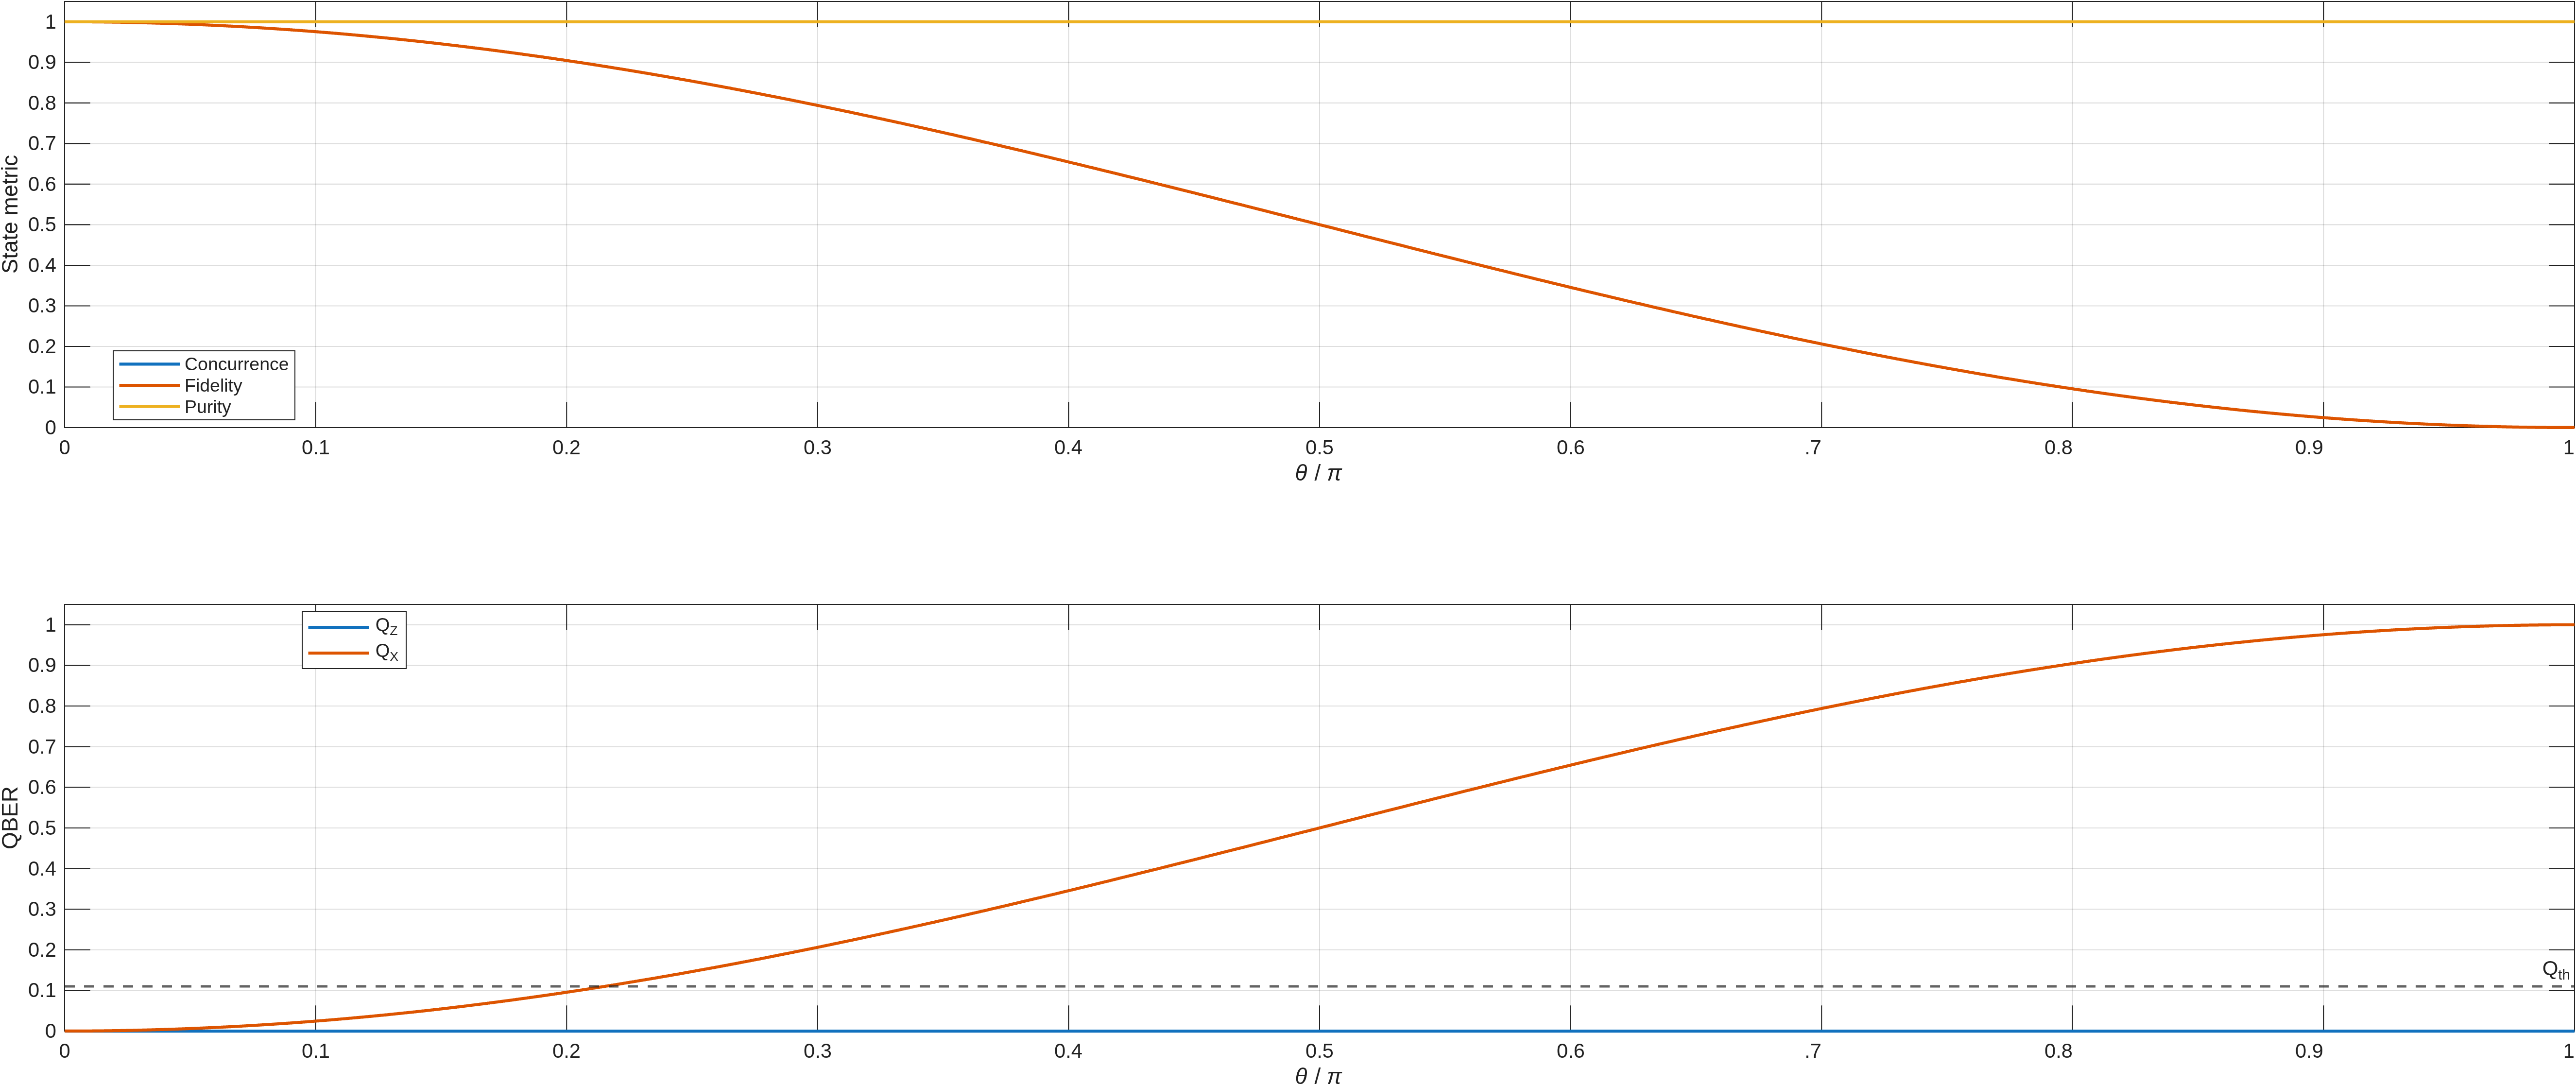
\includegraphics[
        width=0.98\textwidth
    ]{
        figures/experiment_1/phase_summary.png
    }

    \caption{
        Coherent relative-phase evolution. Purity and concurrence remain equal
        to unity, while fidelity and the diagonal-basis QBER vary with the
        relative phase. The dashed line indicates the adopted BBM92 QBER
        threshold.
    }

    \label{fig:exp1_coherent_phase}

\end{figure}

The corresponding numerical operating boundary is

\begin{equation}
\theta_{\mathrm{th}}
\simeq
0.6761~\mathrm{rad}
\simeq
0.215\pi.
\label{eq:exp1_phase_boundary}
\end{equation}

This case directly demonstrates that maximal entanglement does not by itself
guarantee low QBER when measurements are performed in fixed polarization bases.


%--------------------------------------------------------
% Statistical dephasing
%--------------------------------------------------------

\subsection{Statistical Dephasing}

Statistical fluctuations of the relative phase reduce the polarization
coherence. For the real coherence parameter \(\mu\in[0,1]\), the resulting state
is

\begin{equation}
\rho_{\mu}
=
\frac{1}{2}
\left(
|01\rangle\langle 01|
+
|10\rangle\langle 10|
\right)
+
\frac{\mu}{2}
\left(
|01\rangle\langle 10|
+
|10\rangle\langle 01|
\right).
\label{eq:exp1_dephasing_state}
\end{equation}

For this state family,

\begin{equation}
C=\mu,
\qquad
Q_Z=0,
\qquad
Q_X=\frac{1-\mu}{2}.
\label{eq:exp1_dephasing_results}
\end{equation}

As shown in Figure~\ref{fig:exp1_dephasing}, decreasing coherence now corresponds
to genuine entanglement degradation and increasing error in the diagonal basis.

\begin{figure}[htbp]

    \centering

    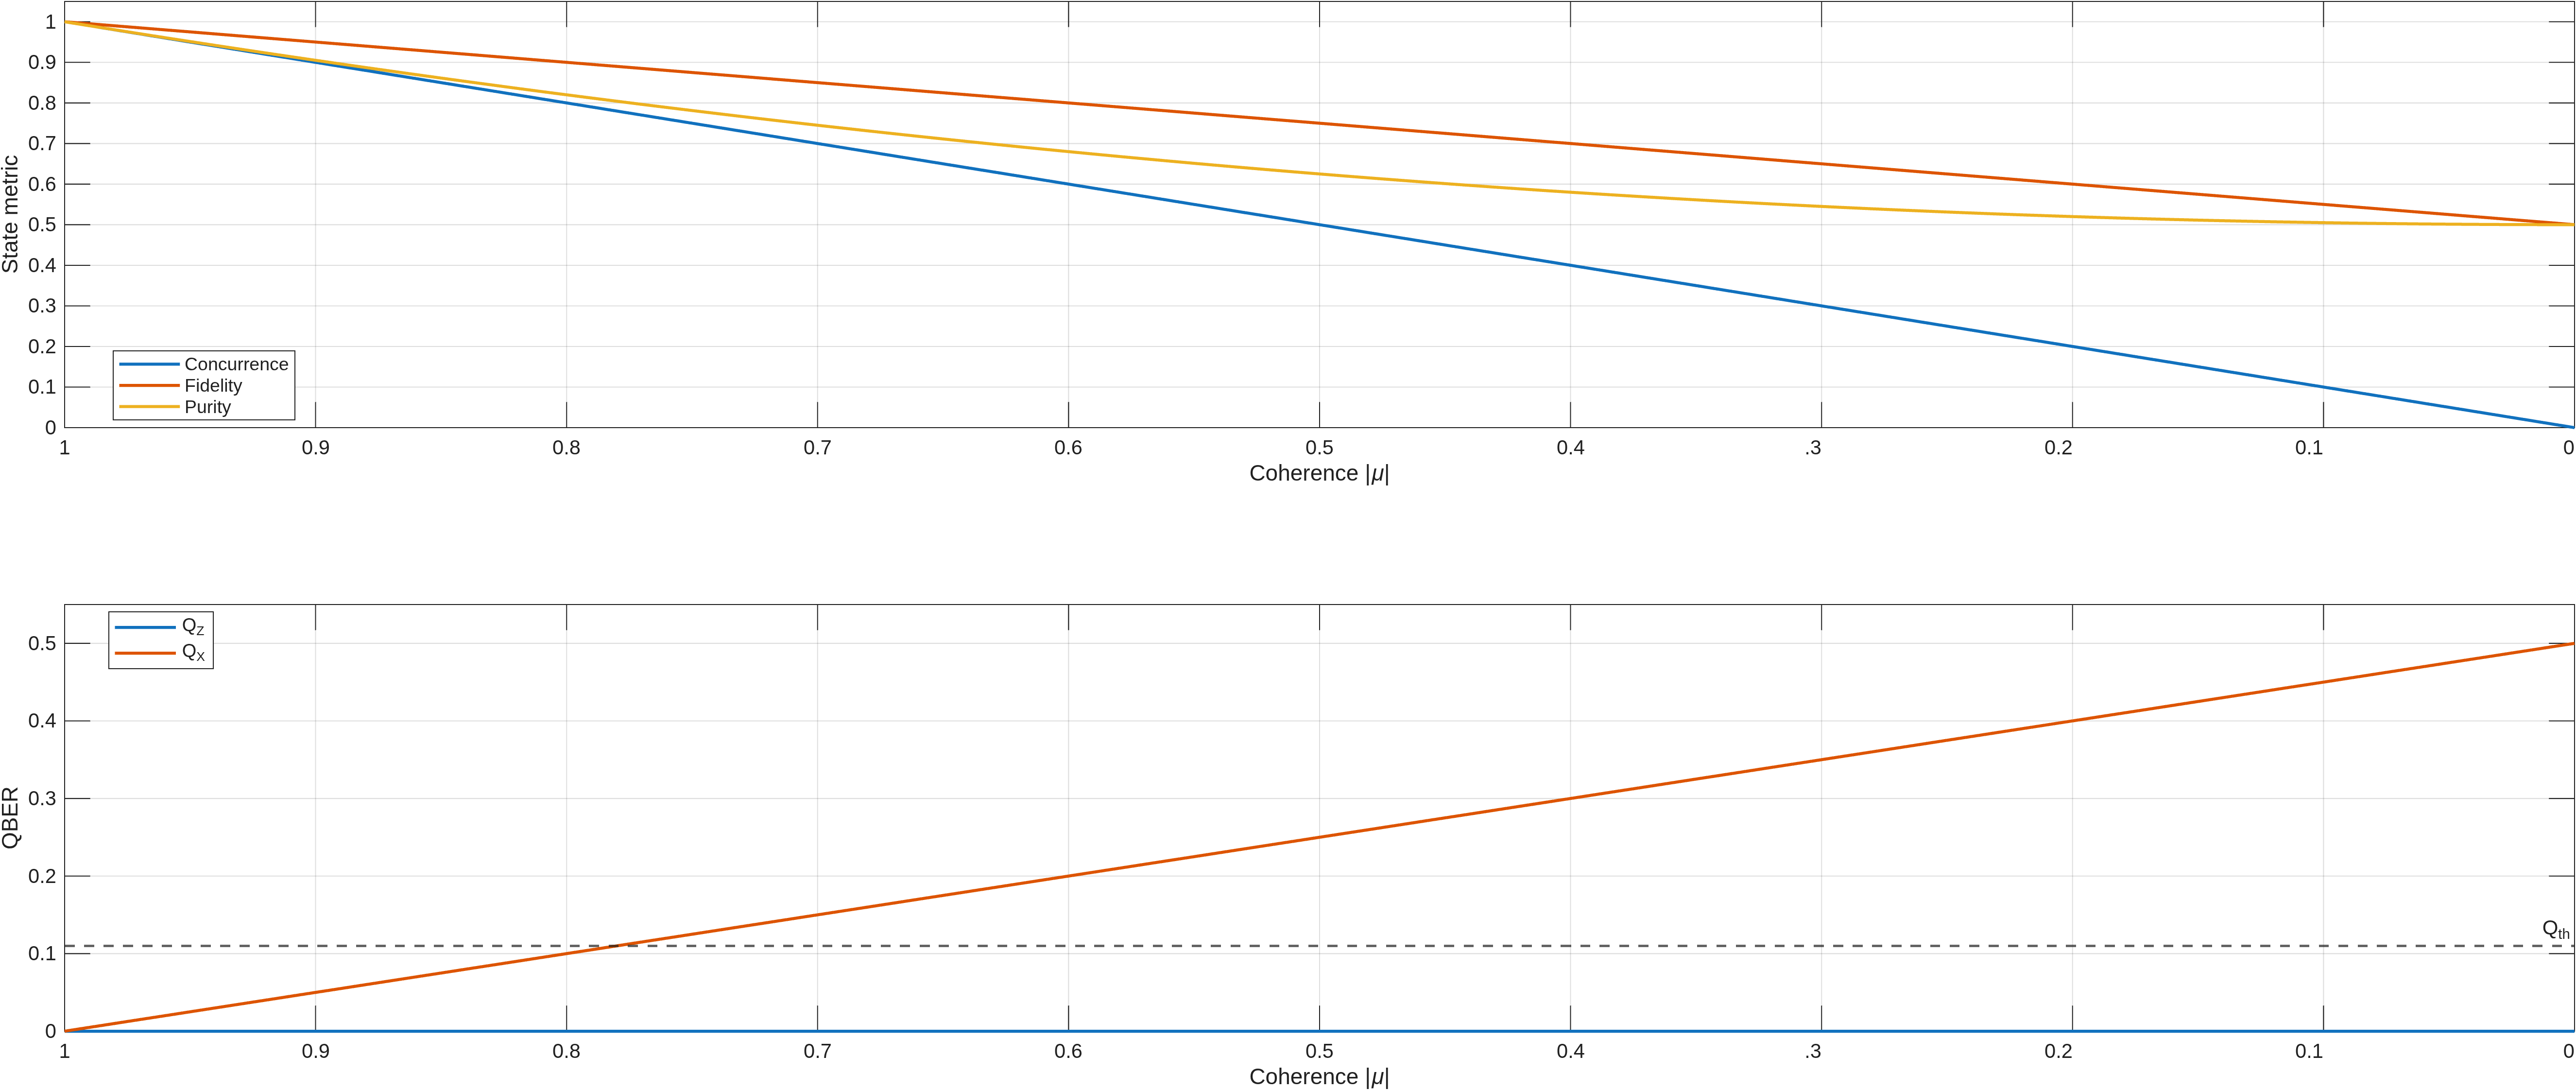
\includegraphics[
        width=0.98\textwidth
    ]{
        figures/experiment_1/dephasing_summary.png
    }

    \caption{
        Statistical dephasing as a function of the coherence parameter
        \(\mu\). Loss of coherence reduces concurrence, purity, and fidelity
        while increasing \(Q_X\); the \(H/V\)-basis correlations remain
        unaffected.
    }

    \label{fig:exp1_dephasing}

\end{figure}

The QBER threshold is crossed at

\begin{equation}
\mu_{\mathrm{th}}
=
0.780.
\label{eq:exp1_dephasing_boundary}
\end{equation}

Because \(C=\mu\) for this particular family, the same point corresponds to
\(C=0.78\). This value is specific to the dephasing model and does not represent
a universal concurrence threshold for BBM92 operation.


%--------------------------------------------------------
% Symmetric local depolarization
%--------------------------------------------------------

\subsection{Symmetric Two-Arm Depolarization}

The third model applies the same local depolarization probability to both
photons,

\begin{equation}
p_A=p_B=p.
\label{eq:exp1_symmetric_depolarization}
\end{equation}

In this case both measurement bases are affected. As shown in
Figure~\ref{fig:exp1_depolarization}, increasing \(p\) progressively decreases
purity, fidelity, and concurrence, while \(Q_Z\) and \(Q_X\) increase together.

\begin{figure}[htbp]

    \centering

    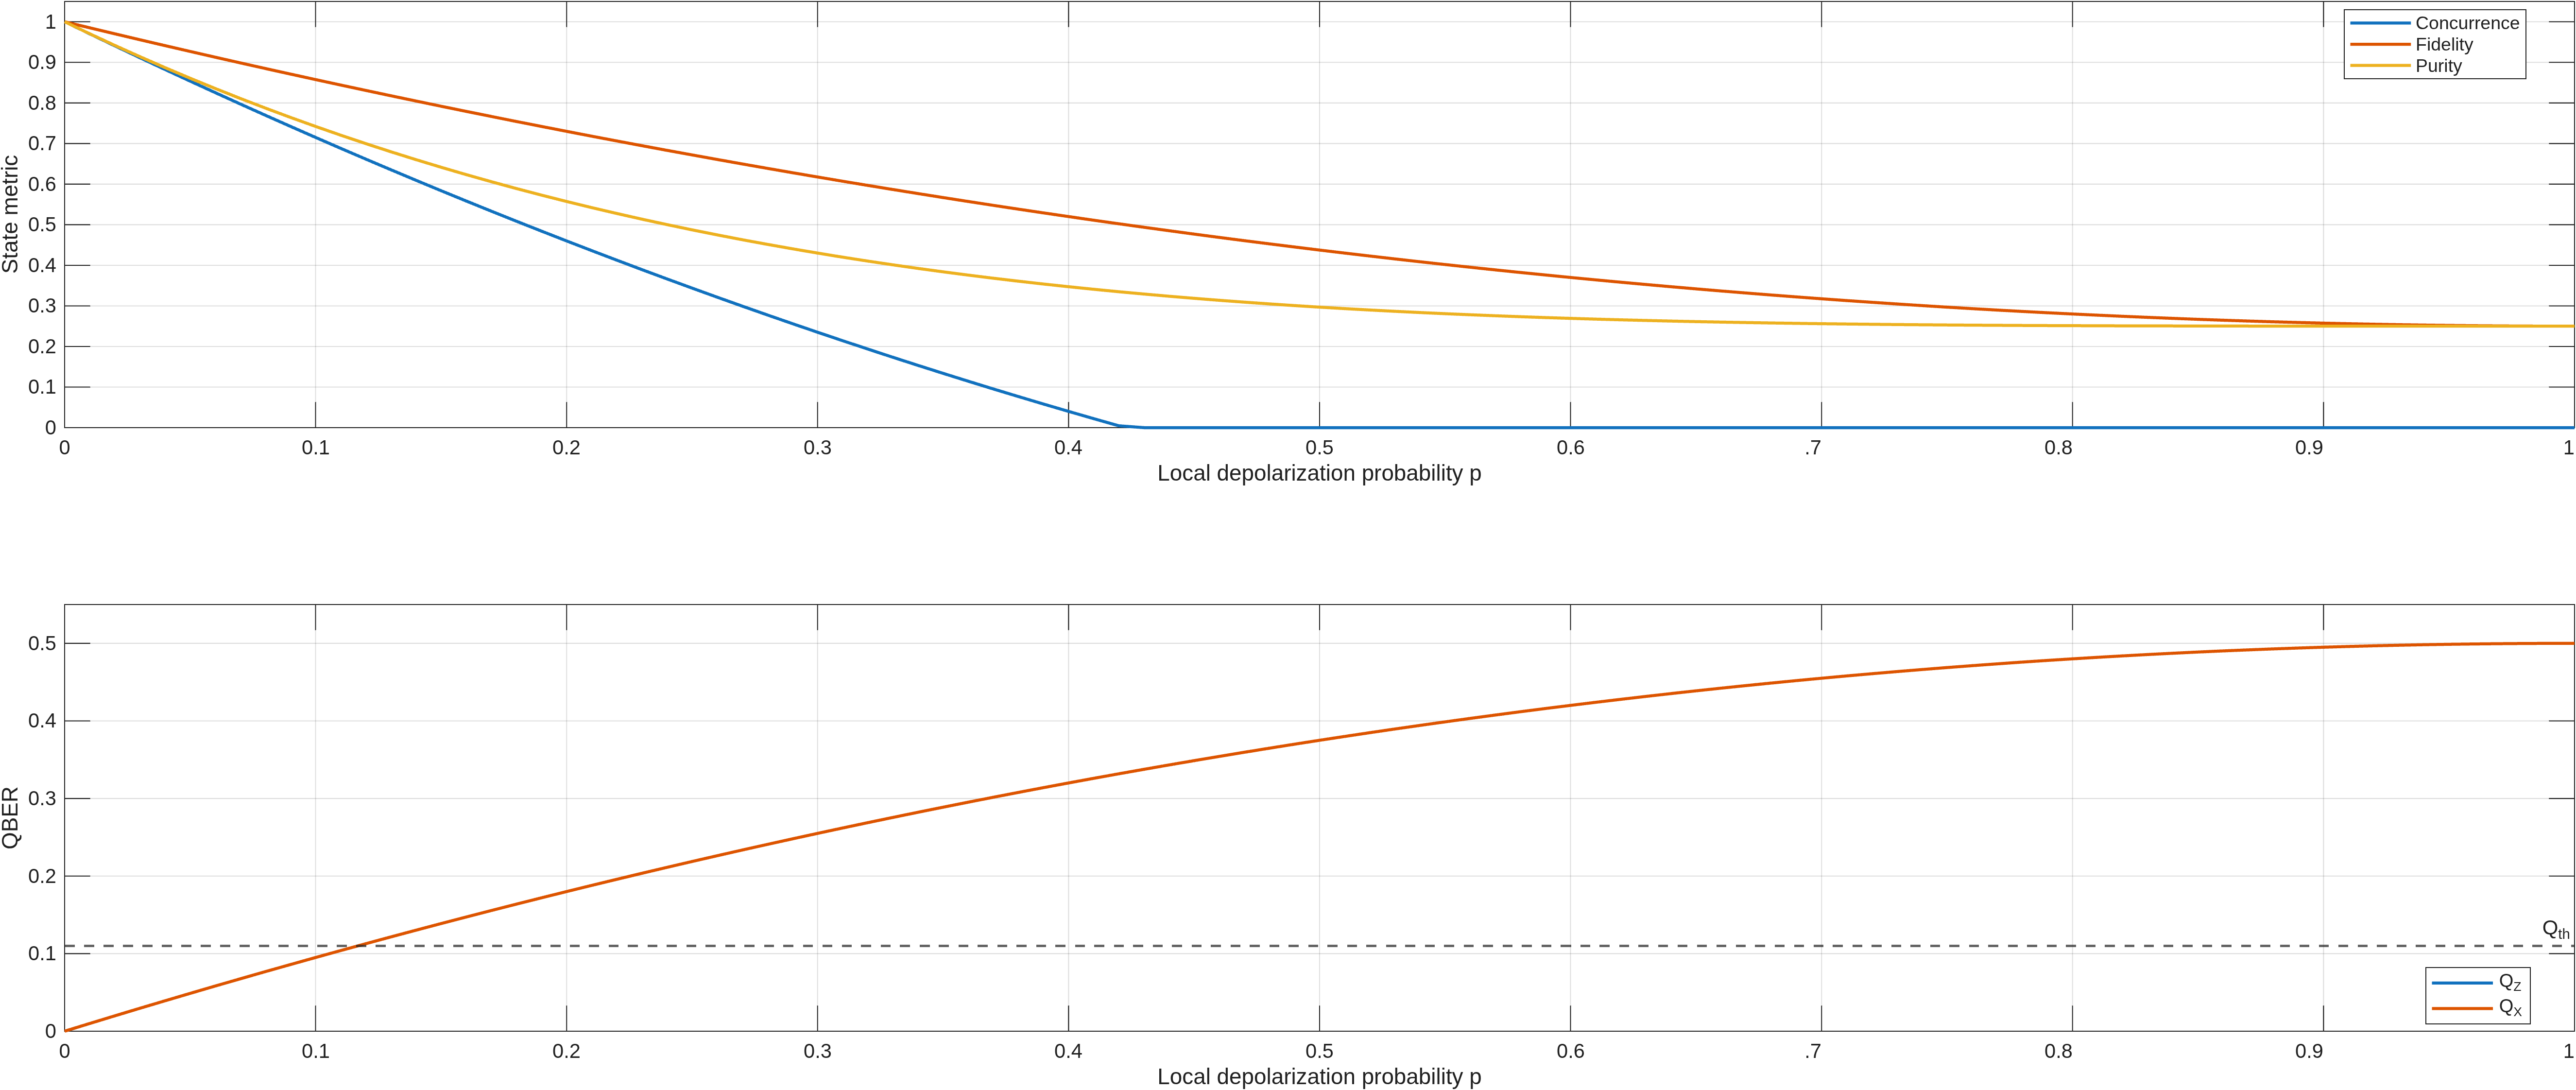
\includegraphics[
        width=0.98\textwidth
    ]{
        figures/experiment_1/depolarization_summary.png
    }

    \caption{
        Symmetric independent local depolarization. Increasing the local
        depolarization probability reduces the state-quality metrics and
        produces equal errors in the two BBM92 measurement bases.
    }

    \label{fig:exp1_depolarization}

\end{figure}

The numerical operating boundary is

\begin{equation}
p_{\mathrm{th}}
\simeq
0.1168.
\label{eq:exp1_depolarization_boundary}
\end{equation}


%--------------------------------------------------------
% Comparison
%--------------------------------------------------------

\subsection{Comparison of State Quality and BBM92 Performance}

Figure~\ref{fig:exp1_concurrence_qber} directly compares the worst-basis QBER
with concurrence for the three models.

\begin{figure}[htbp]

    \centering

    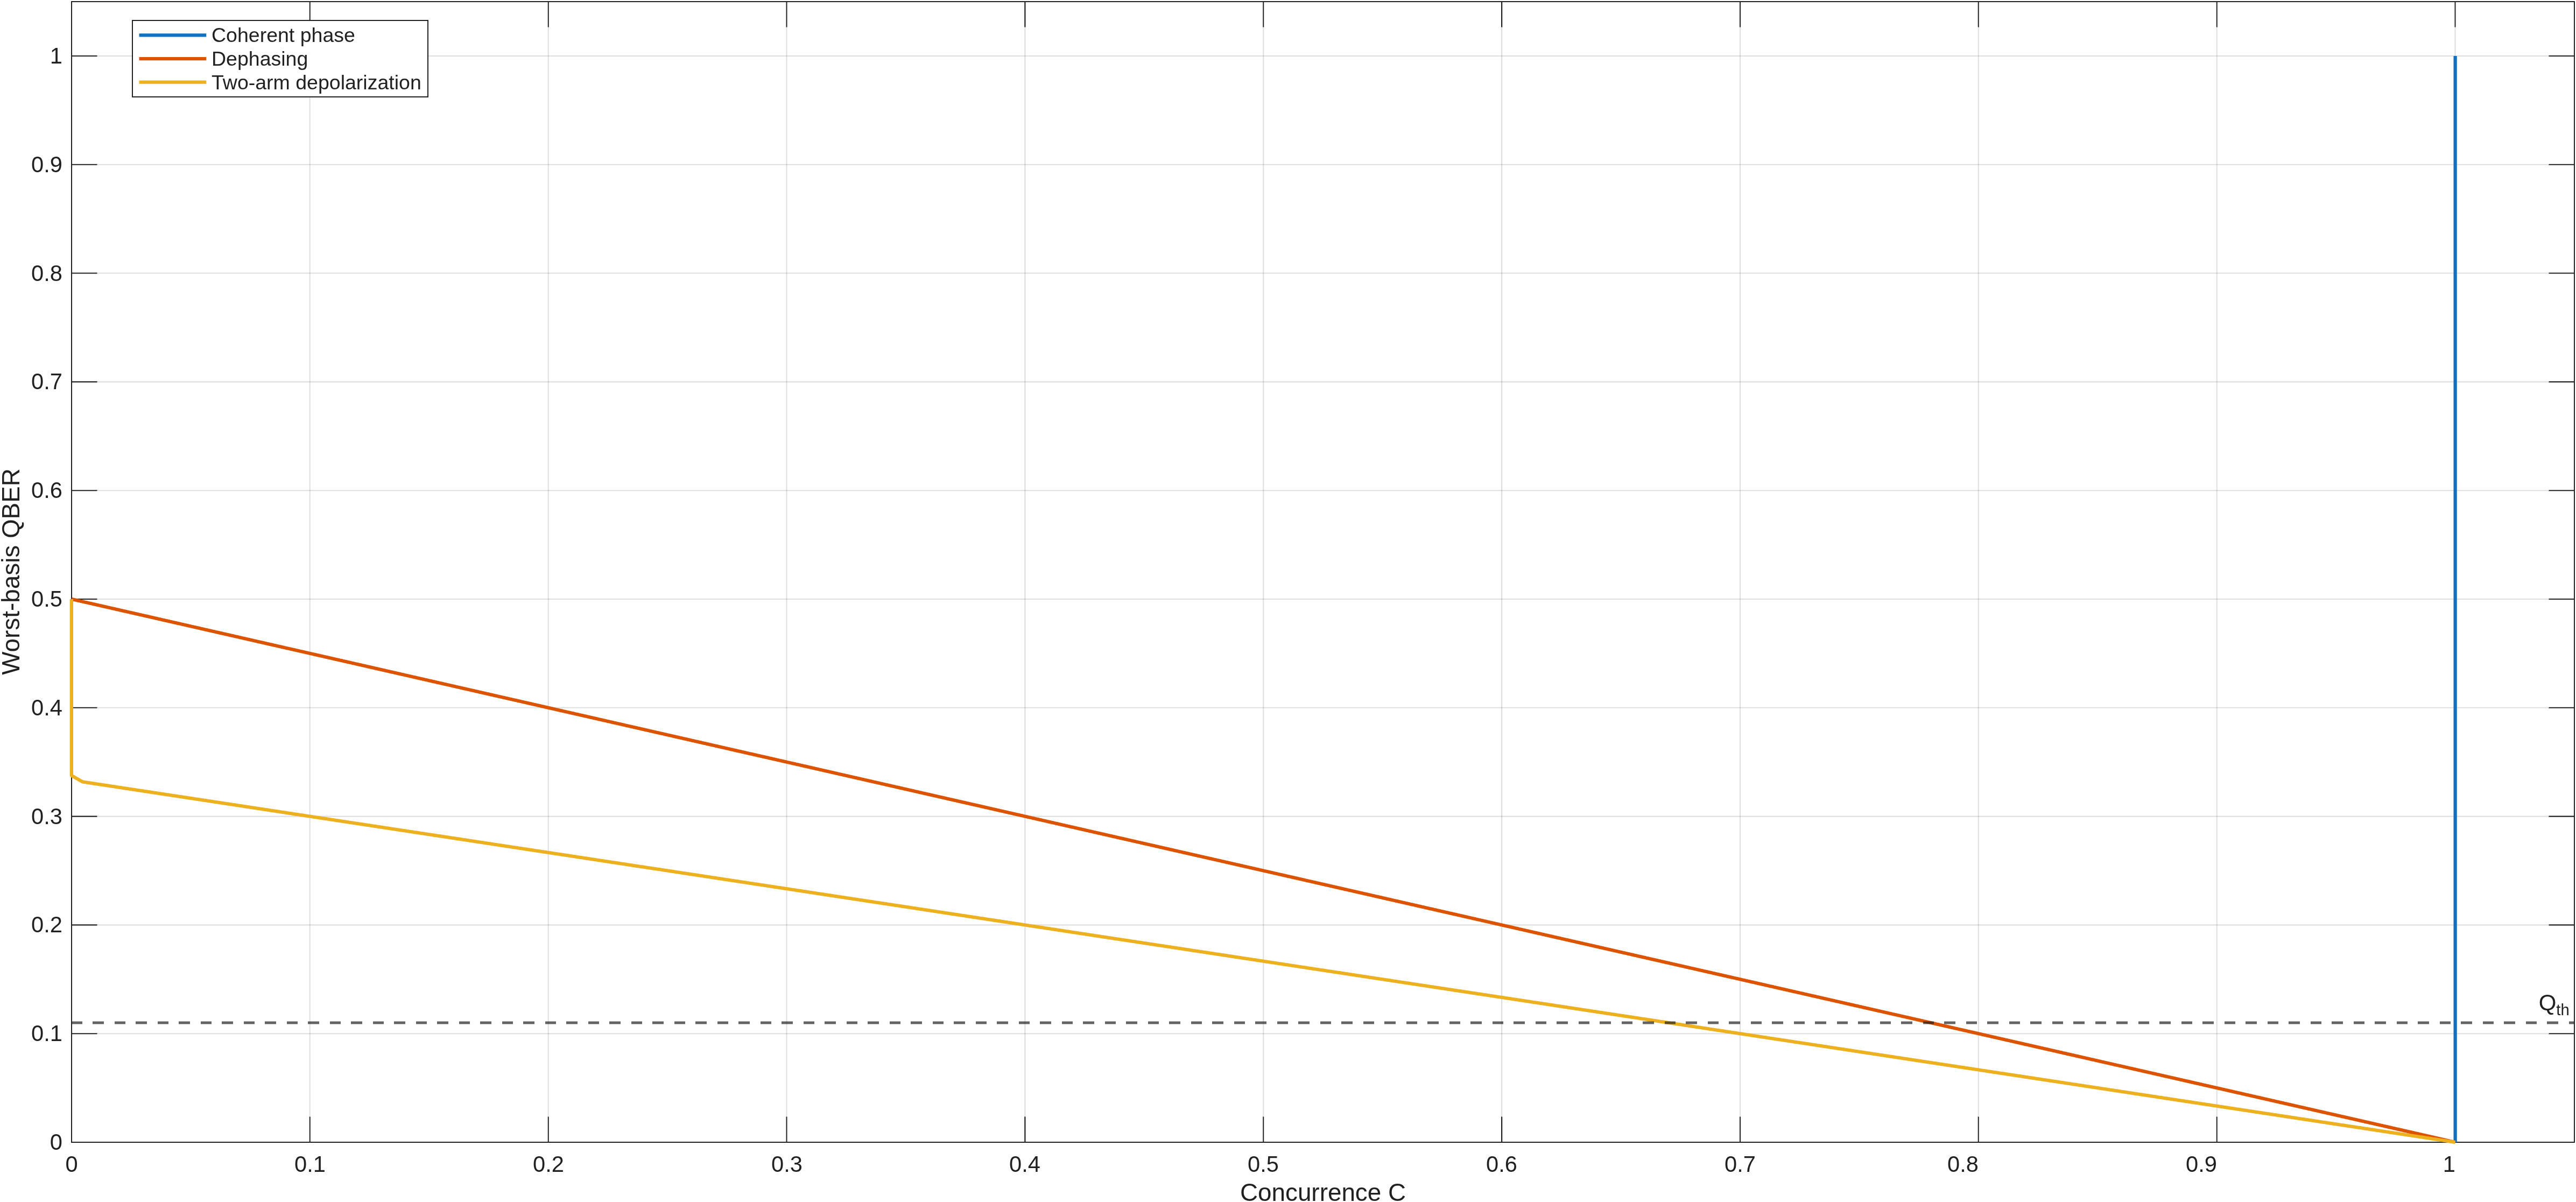
\includegraphics[
        width=0.98\textwidth
    ]{
        figures/experiment_1/concurrence_vs_qber.png
    }

    \caption{
        Worst-basis QBER as a function of concurrence for the three effective
        fiber models. The relation between entanglement and BBM92 performance
        depends on the physical degradation mechanism. Coherent phase evolution
        provides the limiting example in which \(C=1\) while the QBER varies.
    }

    \label{fig:exp1_concurrence_qber}

\end{figure}

The operating boundaries obtained from the three one-parameter models are

\begin{equation}
\boxed{
\theta_{\mathrm{th}}
\simeq
0.6761~\mathrm{rad},
\qquad
\mu_{\mathrm{th}}
=
0.780,
\qquad
p_{\mathrm{th}}
\simeq
0.1168.
}
\label{eq:exp1_boundaries_summary}
\end{equation}

These values parameterize different physical mechanisms and should therefore not
be interpreted as equivalent channel thresholds. Their common meaning is that
they identify where each model crosses the adopted BBM92 QBER criterion.

The experiment establishes the distinction used throughout the following
numerical analysis: purity, fidelity, and concurrence characterize different
properties of the distributed quantum state, whereas the BBM92 operating region
is determined directly from the measurement error rates. The subsequent
experiments extend this criterion from effective channel parameters to the
physical source and fiber parameters of the frequency-dependent propagation
model.

%========================================================
% SECTION 3.3 — Experiment 2
%========================================================

\section{Source--Fiber Operating Region under Single-Arm PMD}
\label{sec:single_arm_pmd_operating_region}
%========================================================
% EXPERIMENT 2 — Source--Fiber Operating Region
%                under Single-Arm PMD
%========================================================

\subsection{Objective and Numerical Setup}

The second numerical experiment introduces the frequency-dependent PMD model and
investigates how the source spectral bandwidth and the fiber differential group
delay jointly determine the BBM92 operating region.

A single-arm configuration is considered in order to isolate this dependence.
The photon propagating through arm \(A\) experiences first-order PMD with a fixed
birefringence axis, while arm \(B\) is kept ideal. The polarization
transformation at the carrier frequency is assumed to be compensated, so that
only the frequency-dependent PMD contribution is retained.

The input polarization state is the reference Bell state \( |\Psi^+\rangle \).
A Gaussian spectral distribution is used, with spectral bandwidth
\(\sigma_\omega\) varied over

\begin{equation}
2.5\times10^{10}
\leq
\sigma_\omega
\leq
2.0\times10^{11}
\;\mathrm{rad/s},
\end{equation}

while the differential group delay is varied over

\begin{equation}
0
\leq
\Delta\tau
\leq
30
\;\mathrm{ps}.
\end{equation}

The numerical spectral integration uses \(81\) frequency nodes per arm over a
window of \(\pm6\sigma_\omega\). The PMD axis in arm \(A\) is chosen along the
\(x\)-axis of the Bloch sphere. With this orientation, the diagonal-basis
correlation is protected, while the computational-basis correlation is degraded
by the frequency-dependent propagation.

For every pair \((\sigma_\omega,\Delta\tau)\), the frequency-resolved
polarization state is propagated and the unresolved spectral degree of freedom
is traced out according to
Eq.~\eqref{eq:pmd_two_arm_reduced_polarization_state}. The resulting polarization
state is characterized through concurrence and the two BBM92 error rates
\(Q_Z\) and \(Q_X\).

The operational classification is based on the worst-basis error

\begin{equation}
Q_{\mathrm{worst}}
=
\max(Q_Z,Q_X),
\label{eq:exp2_worst_basis_qber}
\end{equation}

with the adopted threshold

\begin{equation}
Q_{\mathrm{worst}}
<
Q_{\mathrm{th}},
\qquad
Q_{\mathrm{th}}=0.11.
\label{eq:exp2_operational_condition}
\end{equation}


%--------------------------------------------------------
% Source--Fiber BBM92 Operating Region
%--------------------------------------------------------

\subsection{Source--Fiber BBM92 Operating Region}

Figure~\ref{fig:exp2_single_arm_pmd_operating_region} shows the worst-basis QBER
over the source--fiber parameter space.

\begin{figure}[htbp]
    \centering

    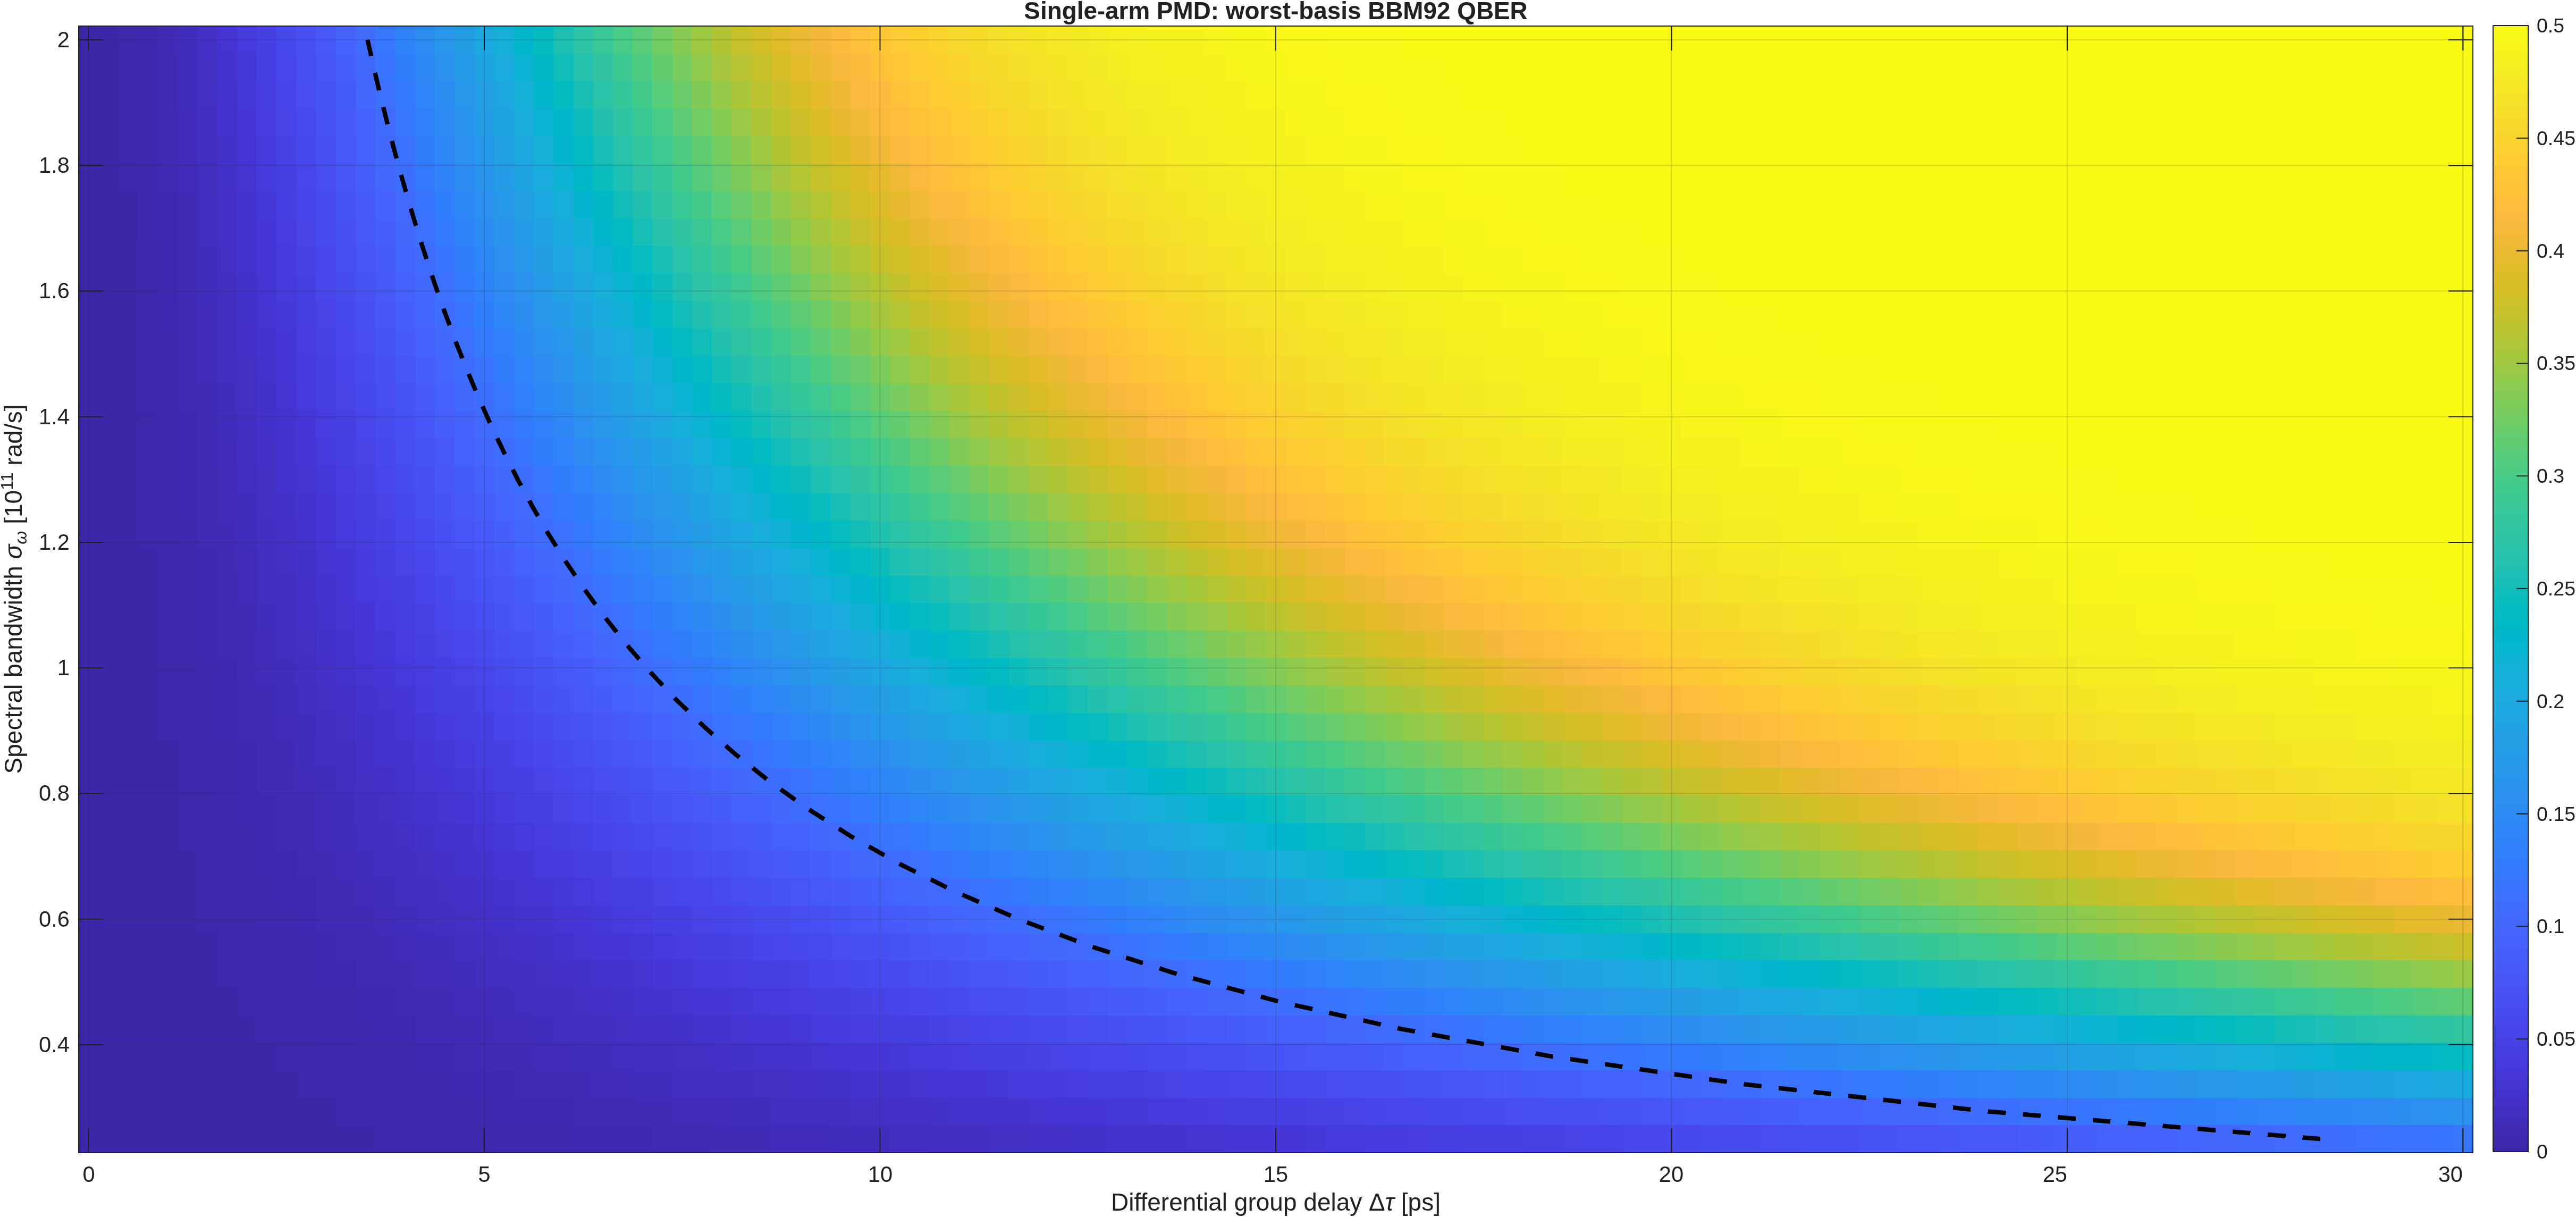
\includegraphics[
        width=0.95\textwidth
    ]{
        figures/experiment_2/single_arm_pmd_operating_region.png
    }

    \caption{
        Worst-basis BBM92 QBER for single-arm first-order PMD as a function of
        the photon spectral bandwidth \(\sigma_\omega\) and the differential
        group delay \(\Delta\tau\). The dashed curve identifies the adopted
        BBM92 operating boundary \(Q_{\mathrm{worst}}=Q_{\mathrm{th}}\), with
        \(Q_{\mathrm{th}}=0.11\).
    }

    \label{fig:exp2_single_arm_pmd_operating_region}
\end{figure}

The operating region lies below and to the left of the dashed boundary. For a
fixed spectral bandwidth, increasing the DGD increases the frequency dependence
of the polarization transformation and consequently the QBER. Conversely, for a
fixed DGD, a broader photon spectrum samples a larger range of
frequency-dependent polarization transformations and therefore produces the same
effect.

The boundary consequently exhibits an approximately inverse dependence between
the maximum tolerable DGD and the source bandwidth. This behavior follows
directly from the normalized PMD parameter introduced in
Eq.~\eqref{eq:normalized_pmd_parameter},

\begin{equation}
\chi
=
\sigma_\omega |\Delta\tau|.
\label{eq:exp2_normalized_pmd_parameter}
\end{equation}

For the Gaussian spectrum considered here, Chapter~\ref{ch:02_fiber_channel_modeling}
showed that the surviving polarization coherence is

\begin{equation}
|\kappa|
=
e^{-\chi^2/2},
\end{equation}

as given by Eq.~\eqref{eq:gaussian_pmd_coherence_normalized}. The numerical
operating boundary is therefore expected to correspond to an approximately
constant value of \(\chi\), rather than to an independent limitation on
\(\sigma_\omega\) or \(\Delta\tau\).


%--------------------------------------------------------
% Entanglement at the Operational Boundary
%--------------------------------------------------------

\subsection{Entanglement at the Operational Boundary}

The corresponding concurrence is shown in
Fig.~\ref{fig:exp2_single_arm_pmd_concurrence}. The same BBM92 operating boundary
is superimposed on the state-quality map.

\begin{figure}[htbp]
    \centering

    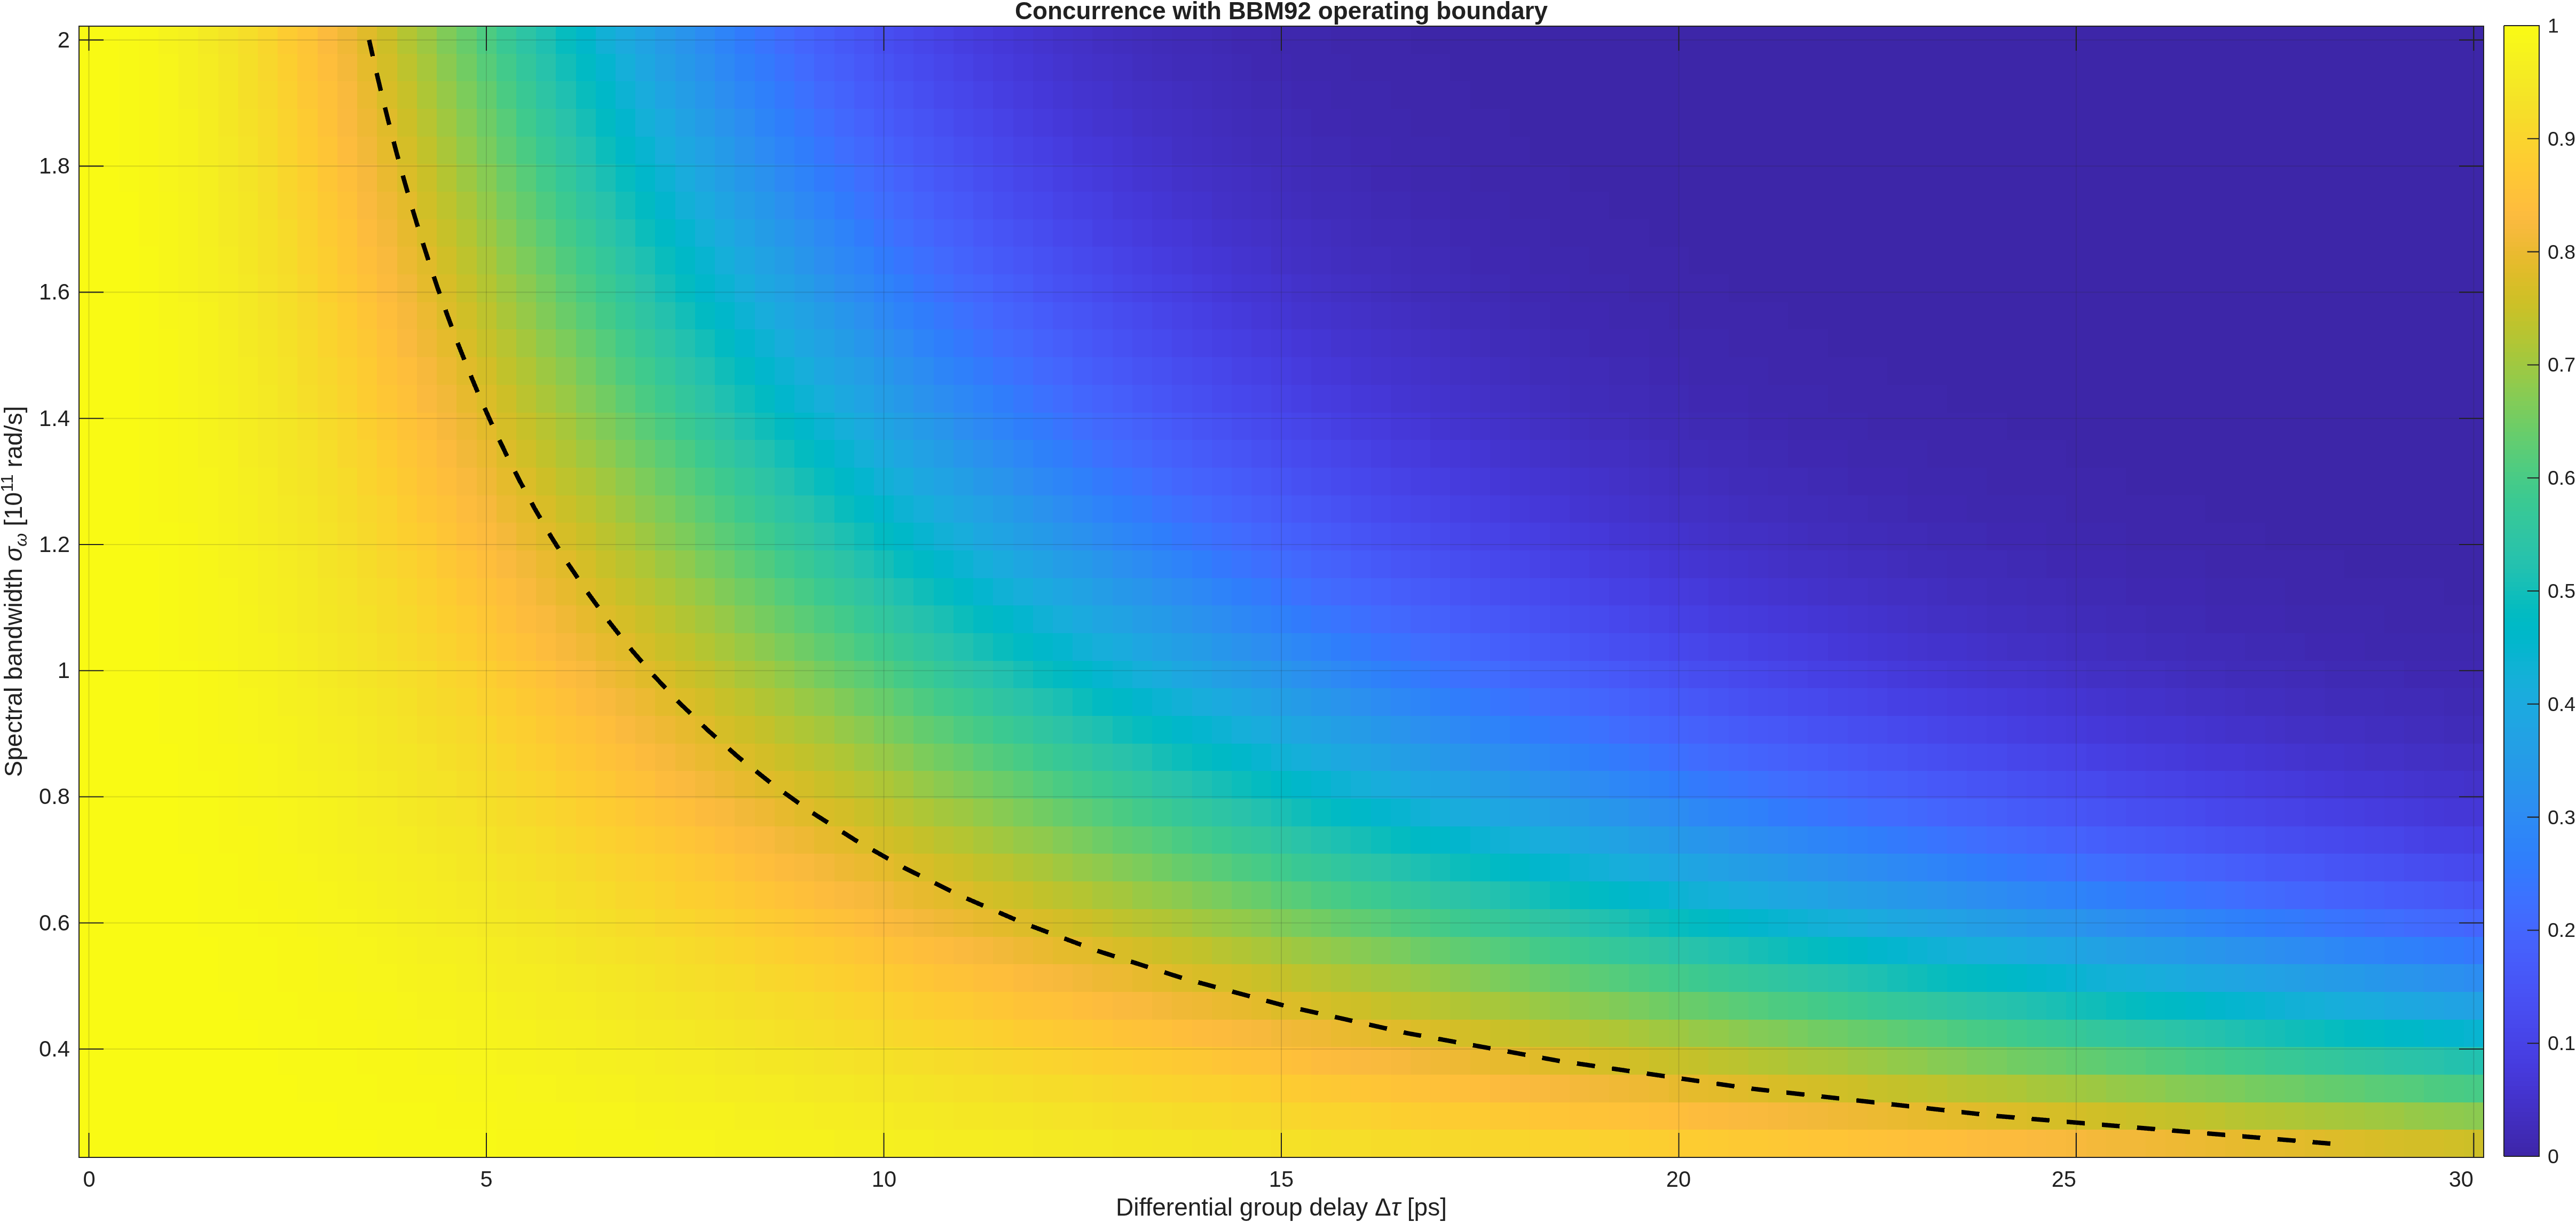
\includegraphics[
        width=0.95\textwidth
    ]{
        figures/experiment_2/single_arm_pmd_concurrence_map.png
    }

    \caption{
        Concurrence of the reduced polarization state under single-arm
        first-order PMD. The dashed curve is the BBM92 operating boundary
        obtained from \(Q_{\mathrm{worst}}=0.11\), rather than from an imposed
        concurrence threshold.
    }

    \label{fig:exp2_single_arm_pmd_concurrence}
\end{figure}

The concurrence decreases continuously as the product
\(\sigma_\omega|\Delta\tau|\) increases. This behavior is consistent with the
analytical single-arm Gaussian result derived in
Eq.~\eqref{eq:single_arm_pmd_concurrence_analytical},

\begin{equation}
C(\chi)
=
e^{-\chi^2/2}.
\end{equation}

Importantly, the dashed curve in
Fig.~\ref{fig:exp2_single_arm_pmd_concurrence} is not defined by selecting an
independent minimum acceptable concurrence. It is obtained exclusively from the
BBM92 QBER requirement and subsequently represented on the concurrence map.
The figure therefore shows the amount of entanglement remaining when the
operational QBER boundary is reached.


%--------------------------------------------------------
% Numerical and Analytical Boundary
%--------------------------------------------------------

\subsection{Operating-Boundary Analysis}

The numerical results confirm that the source bandwidth and fiber DGD enter the
operational boundary predominantly through the normalized PMD parameter
\(\chi=\sigma_\omega|\Delta\tau|\).

For the adopted QBER threshold, the analytical single-arm Gaussian model gives

\begin{equation}
\chi_{\mathrm{th}}^{\mathrm{ana}}
=
0.704927.
\label{eq:exp2_analytical_chi_threshold}
\end{equation}

The numerical parameter sweep gives

\begin{equation}
\overline{\chi}_{\mathrm{th}}^{\mathrm{num}}
=
0.704872,
\qquad
\sigma_{\chi_{\mathrm{th}}}
=
5.505\times10^{-5},
\label{eq:exp2_numerical_chi_threshold}
\end{equation}

with a maximum absolute deviation from the analytical boundary of

\begin{equation}
\max
\left|
\chi_{\mathrm{th}}^{\mathrm{num}}
-
\chi_{\mathrm{th}}^{\mathrm{ana}}
\right|
=
2.044\times10^{-4}.
\label{eq:exp2_chi_boundary_error}
\end{equation}

The concurrence evaluated along the numerical BBM92 boundary is correspondingly

\begin{equation}
\overline{C}_{\mathrm{th}}
=
0.780000,
\end{equation}

with a standard deviation of only \(1.902\times10^{-9}\) over the explored
bandwidth range. The approximately constant concurrence along the boundary is a
consequence of the single-parameter dependence of this particular fixed-axis
Gaussian PMD model and should therefore not be interpreted as a universal
concurrence threshold for BBM92 operation.

The simulation also reproduces the expected limiting behavior at zero DGD:
the propagated state remains the original Bell state, with unit concurrence and
zero QBER in both measurement bases. For the selected \(x\)-oriented PMD axis,
the diagonal basis remains protected throughout the sweep,
\(Q_X=0\), while \(Q_Z\) determines the operating boundary.

The experiment therefore reduces the two-dimensional source--fiber parameter
space to a physically meaningful normalized condition,

\begin{equation}
\boxed{
\sigma_\omega|\Delta\tau|
<
\chi_{\mathrm{th}}
\simeq
0.705,
}
\label{eq:exp2_final_operational_condition}
\end{equation}

for the specific single-arm, fixed-axis, Gaussian PMD configuration considered
here. This result provides the first direct source--fiber operating map of the
numerical analysis and establishes the reference case for the two-arm and
spectrally correlated configurations considered in the following experiment.

%========================================================
% SECTION 3.4 — Experiment 3
%========================================================

\section{Two-Arm PMD and Spectral-Correlation Operating Regions}
\label{sec:two_arm_pmd_spectral_operating_regions}
%========================================================
% EXPERIMENT 3 — Two-Arm PMD and Spectral-Correlation
%                Operating Regions
%========================================================

\subsection{Objective and Numerical Setup}

The third numerical experiment extends the single-arm analysis of
Section~\ref{sec:single_arm_pmd_operating_region} to the complete two-arm
configuration. The objective is to determine how PMD accumulated by both photons
combines with the spectral correlations of the entangled-photon source in
determining the BBM92 operating region.

The frequency offsets of photons \(A\) and \(B\) from their respective carrier
frequencies are denoted by

\begin{equation}
\Omega_A
=
\omega_A-\omega_{0,A},
\qquad
\Omega_B
=
\omega_B-\omega_{0,B}.
\label{eq:exp3_frequency_offsets}
\end{equation}

The joint spectral statistics of the two photons are described by a Gaussian
joint spectral intensity of the form

\begin{equation}
J(\Omega_A,\Omega_B)
\propto
\exp
\left[
-
\frac{(\Omega_A+\Omega_B)^2}
     {2\sigma_{\Sigma}^{\,2}}
-
\frac{(\Omega_A-\Omega_B)^2}
     {2\sigma_{\Delta}^{\,2}}
\right],
\label{eq:exp3_gaussian_jsi}
\end{equation}

where \(\sigma_{\Sigma}\) and \(\sigma_{\Delta}\) control the widths along the
sum- and difference-frequency directions, respectively.

For equal marginal spectral bandwidths,

\begin{equation}
\sigma_{\omega,A}
=
\sigma_{\omega,B}
=
\sigma_\omega,
\end{equation}

the spectral correlation coefficient is defined as

\begin{equation}
\boxed{
r
=
\frac{
\operatorname{Cov}(\Omega_A,\Omega_B)
}{
\sigma_\omega^2
},
\qquad
-1<r<1.
}
\label{eq:exp3_spectral_correlation_coefficient}
\end{equation}

With the Gaussian convention adopted in the simulator, the corresponding
sum- and difference-frequency widths are

\begin{equation}
\sigma_{\Sigma}
=
\sigma_\omega
\sqrt{2(1+r)},
\qquad
\sigma_{\Delta}
=
\sigma_\omega
\sqrt{2(1-r)}.
\label{eq:exp3_joint_spectral_widths}
\end{equation}

The parameter \(r\) therefore describes how the frequency offsets of the two
photons are statistically related. For \(r<0\), the frequencies are
anticorrelated: a positive frequency offset of one photon tends to be accompanied
by a negative offset of the other. For \(r>0\), the two offsets tend to have the
same sign and are positively correlated. The case \(r=0\) corresponds to
statistically uncorrelated frequency offsets.

Equivalently, negative \(r\) narrows the distribution along the
sum-frequency coordinate \(\Omega_A+\Omega_B\), whereas positive \(r\) narrows
it along the difference-frequency coordinate \(\Omega_A-\Omega_B\). The joint
spectral distribution therefore determines which combinations of photon
frequencies contribute most strongly to the propagated two-photon state.


%--------------------------------------------------------
% Frequency-Resolved Two-Photon States
%--------------------------------------------------------

\subsection{Generation of the Frequency-Resolved Polarization States}

The input polarization state is the Bell state

\begin{equation}
|\Psi^{+}\rangle
=
\frac{1}{\sqrt{2}}
\left(
|01\rangle+|10\rangle
\right),
\nonumber
\end{equation}

with density operator

\begin{equation}
\rho_{\mathrm{in}}
=
\ket{\Psi^+}
\bra{\Psi^+}.
\nonumber
\end{equation}

For every spectral pair
\((\Omega_A,\Omega_B)\), the polarization state is propagated through the two
frequency-dependent fiber transformations according to

\begin{equation}
\rho_{AB}(\Omega_A,\Omega_B)
=
U_{AB}(\Omega_A,\Omega_B)
\rho_{\mathrm{in}}
U_{AB}^{\dagger}(\Omega_A,\Omega_B),
\label{eq:exp3_frequency_resolved_state}
\end{equation}

where

\begin{equation}
U_{AB}(\Omega_A,\Omega_B)
=
U_A(\Omega_A)
\otimes
U_B(\Omega_B).
\label{eq:exp3_two_arm_unitary}
\end{equation}

Each arm is represented by one first-order PMD segment. Using the fiber model
introduced in Chapter~\ref{ch:02_fiber_channel_modeling}, the corresponding
unitary is

\begin{equation}
U_K(\Omega_K)
=
\exp
\left[
\frac{i}{2}
\Delta\tau_K
\Omega_K
\left(
\mathbf{n}_K\cdot\boldsymbol{\sigma}
\right)
\right],
\qquad
K\in\{A,B\},
\label{eq:exp3_single_arm_pmd_unitary}
\end{equation}

where \(\Delta\tau_K\) is the differential group delay and
\(\mathbf{n}_K\) is the local birefringence axis. The carrier-frequency
differential phase is set to zero in the present experiment so that only the
frequency-dependent PMD contribution is retained.

Both PMD axes are fixed along the same direction,

\begin{equation}
\mathbf{n}_A
=
\mathbf{n}_B
=
\hat{\mathbf{x}},
\label{eq:exp3_aligned_pmd_axes}
\end{equation}

so that the experiment isolates the effects of
\(\Delta\tau_A\), \(\Delta\tau_B\), and the spectral correlation \(r\).
Relative PMD-axis misalignment is investigated separately in the following
experiment.

The joint spectral distribution in
Eq.~\eqref{eq:exp3_gaussian_jsi} generates a statistical ensemble of
frequency-resolved polarization states. Since the photon frequencies are not
resolved in the polarization measurement, the reduced polarization density
operator is obtained by tracing over the spectral degree of freedom,

\begin{equation}
\boxed{
\rho_{\mathrm{pol}}
=
\iint
d\Omega_A\,d\Omega_B\,
P(\Omega_A,\Omega_B)
\rho_{AB}(\Omega_A,\Omega_B),
}
\label{eq:exp3_spectral_average}
\end{equation}

where

\begin{equation}
P(\Omega_A,\Omega_B)
=
\frac{
J(\Omega_A,\Omega_B)
}{
\displaystyle
\iint
d\Omega_A\,d\Omega_B\,
J(\Omega_A,\Omega_B)
}
\label{eq:exp3_normalized_jsi}
\end{equation}

is the normalized joint spectral probability distribution.

Numerically, the integral in Eq.~\eqref{eq:exp3_spectral_average} is evaluated
over the discrete spectral grid as

\begin{equation}
\rho_{\mathrm{pol}}
\simeq
\sum_{k,l}
Q_{kl}
\rho_{AB}
\left(
\Omega_{A,k},
\Omega_{B,l}
\right),
\label{eq:exp3_discrete_spectral_trace}
\end{equation}

where \(Q_{kl}\) are the normalized quadrature-weighted probabilities generated
from the Gaussian joint spectral intensity.

This construction makes the physical role of the source spectrum explicit.
Different values of \(r\) generate different statistical combinations of
\((\Omega_A,\Omega_B)\), which are subsequently converted by the two fiber
transformations into different distributions of polarization transformations.
The reduced polarization state therefore depends jointly on the source spectrum
and on the PMD parameters of both fiber arms.


%--------------------------------------------------------
% Physical Role of Spectral Correlation
%--------------------------------------------------------

\subsection{Physical Role of Spectral Correlation}

For the first-order model of Eq.~\eqref{eq:exp3_single_arm_pmd_unitary}, the
frequency-dependent differential phases accumulated in the two arms scale as

\begin{equation}
\delta\phi_A
=
\Delta\tau_A\Omega_A,
\qquad
\delta\phi_B
=
\Delta\tau_B\Omega_B.
\label{eq:exp3_two_arm_pmd_phases}
\end{equation}

Consequently, correlations between \(\Omega_A\) and \(\Omega_B\) translate
directly into correlations between the PMD-induced phase contributions.

For \(r<0\), the two frequency offsets preferentially have opposite signs.
When the two DGDs are comparable and the PMD axes are aligned, the corresponding
frequency-dependent contributions can therefore partially compensate. For
\(r>0\), the frequency offsets preferentially vary in the same direction and the
two PMD contributions instead tend to reinforce each other.

The two-arm PMD degradation is consequently determined not only by the
individual values of \(\Delta\tau_A\) and \(\Delta\tau_B\), but also by the
joint spectral structure of the photon pair. This is the principal physical
difference with respect to the single-arm configuration investigated in the
previous experiment.


%--------------------------------------------------------
% Numerical Parameter Space
%--------------------------------------------------------

\subsection{Numerical Parameter Space}

The marginal spectral bandwidth is fixed to

\begin{equation}
\sigma_\omega
=
1.0\times10^{11}
\;\mathrm{rad/s}.
\label{eq:exp3_sigma_omega}
\end{equation}

The two differential group delays are independently varied over

\begin{equation}
0
\leq
\Delta\tau_A,\Delta\tau_B
\leq
20
\;\mathrm{ps},
\end{equation}

using \(31\) points per arm.

Three representative spectral-correlation conditions are initially considered,

\begin{equation}
r=-0.9,
\qquad
r=0,
\qquad
r=+0.9,
\label{eq:exp3_representative_correlations}
\end{equation}

corresponding respectively to strongly anticorrelated, uncorrelated, and
strongly positively correlated spectra.

The spectral trace is evaluated using \(41\) frequency nodes per arm over the
interval

\begin{equation}
-6\sigma_\omega
\leq
\Omega_K
\leq
6\sigma_\omega.
\end{equation}

A second numerical sweep varies the spectral correlation continuously over

\begin{equation}
-0.9
\leq
r
\leq
0.9
\end{equation}

using \(37\) points, while restricting the fiber parameters to the symmetric
configuration

\begin{equation}
\Delta\tau_A
=
\Delta\tau_B
=
\Delta\tau.
\label{eq:exp3_symmetric_dgd_condition}
\end{equation}

For each resulting reduced polarization state, the basis-dependent BBM92 error
rates are evaluated and the operational metric is defined as

\begin{equation}
Q_{\mathrm{worst}}
=
\max
\left(
Q_Z,Q_X
\right).
\label{eq:exp3_worst_qber}
\end{equation}

The adopted operating condition is

\begin{equation}
\boxed{
Q_{\mathrm{worst}}
<
0.11.
}
\label{eq:exp3_bbm92_condition}
\end{equation}


%--------------------------------------------------------
% Two-Arm Operating Regions
%--------------------------------------------------------

\subsection{Two-Arm Operating Regions}

Figure~\ref{fig:exp3_two_arm_operating_regions} shows the resulting worst-basis
QBER in the \((\Delta\tau_A,\Delta\tau_B)\) plane for the three representative
spectral-correlation conditions.

\begin{figure}[htbp]
    \centering

    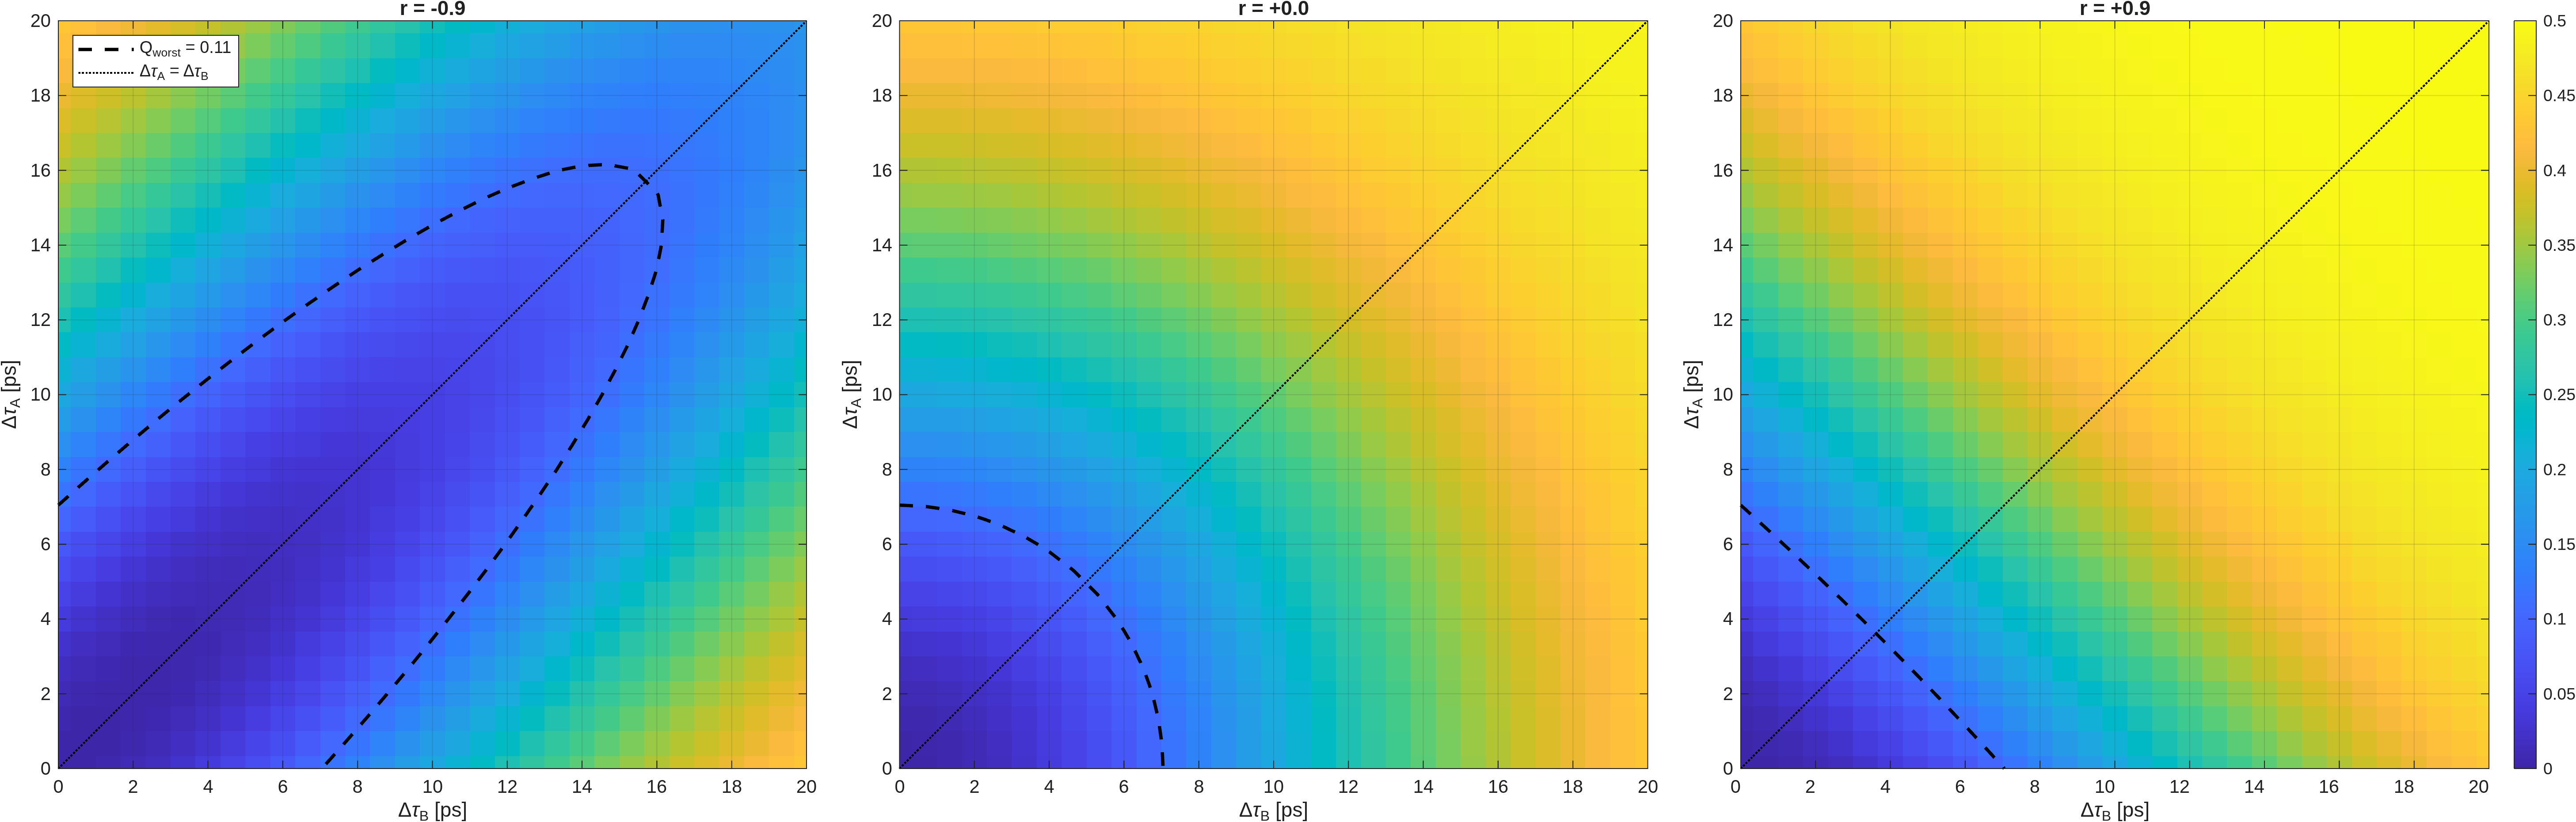
\includegraphics[
        width=\textwidth
    ]{
        figures/experiment_3/two_arm_pmd_operating_regions.png
    }

    \caption{
        Worst-basis BBM92 QBER as a function of the differential group delays
        \(\Delta\tau_A\) and \(\Delta\tau_B\) for strongly anticorrelated
        (\(r=-0.9\)), uncorrelated (\(r=0\)), and strongly positively
        correlated (\(r=+0.9\)) photon spectra. The dashed contour identifies
        the adopted operating boundary \(Q_{\mathrm{worst}}=0.11\), while the
        dotted line denotes the symmetric condition
        \(\Delta\tau_A=\Delta\tau_B\).
    }

    \label{fig:exp3_two_arm_operating_regions}
\end{figure}

The three panels show that spectral correlation changes not only the magnitude
of PMD-induced degradation but also the geometry of the two-arm operating
region.

For \(r=0\), the frequency offsets of the two photons are statistically
uncorrelated. Increasing the DGD in either arm therefore progressively increases
the effective polarization degradation, and the BBM92 operating region remains
concentrated around configurations in which the two DGDs are sufficiently
small.

For \(r=+0.9\), the two frequency offsets tend to have the same sign. For the
aligned PMD configuration considered here, the corresponding
frequency-dependent contributions tend to reinforce each other. The operating
region is consequently reduced when both arms simultaneously exhibit
significant DGD.

A qualitatively different behavior is observed for \(r=-0.9\). The frequency
offsets now preferentially have opposite signs. When the DGDs are comparable,
the two PMD-induced contributions can partially compensate. The BBM92 operating
region therefore extends toward substantially larger DGDs in the vicinity of

\begin{equation}
\Delta\tau_A
\simeq
\Delta\tau_B.
\end{equation}

The diagonal extension visible in the left panel is therefore a direct
consequence of the interaction between the anticorrelated source spectrum and
the frequency-dependent transformations of the two fiber arms. In particular,
large individual DGDs do not necessarily imply a correspondingly large
polarization degradation when their effects are correlated through the joint
spectrum.


%--------------------------------------------------------
% Symmetric-DGD Operating Boundary
%--------------------------------------------------------

\subsection{Spectral Correlation and Symmetric-DGD Tolerance}

The influence of spectral correlation is quantified more directly by restricting
the two-arm parameter space to

\begin{equation}
\Delta\tau_A
=
\Delta\tau_B
=
\Delta\tau
\end{equation}

and determining, for every value of \(r\), the maximum DGD compatible with the
adopted BBM92 criterion.

The resulting threshold
\(\Delta\tau_{\mathrm{th}}\) is shown in
Fig.~\ref{fig:exp3_spectral_correlation_boundary}.

\begin{figure}[htbp]
    \centering

    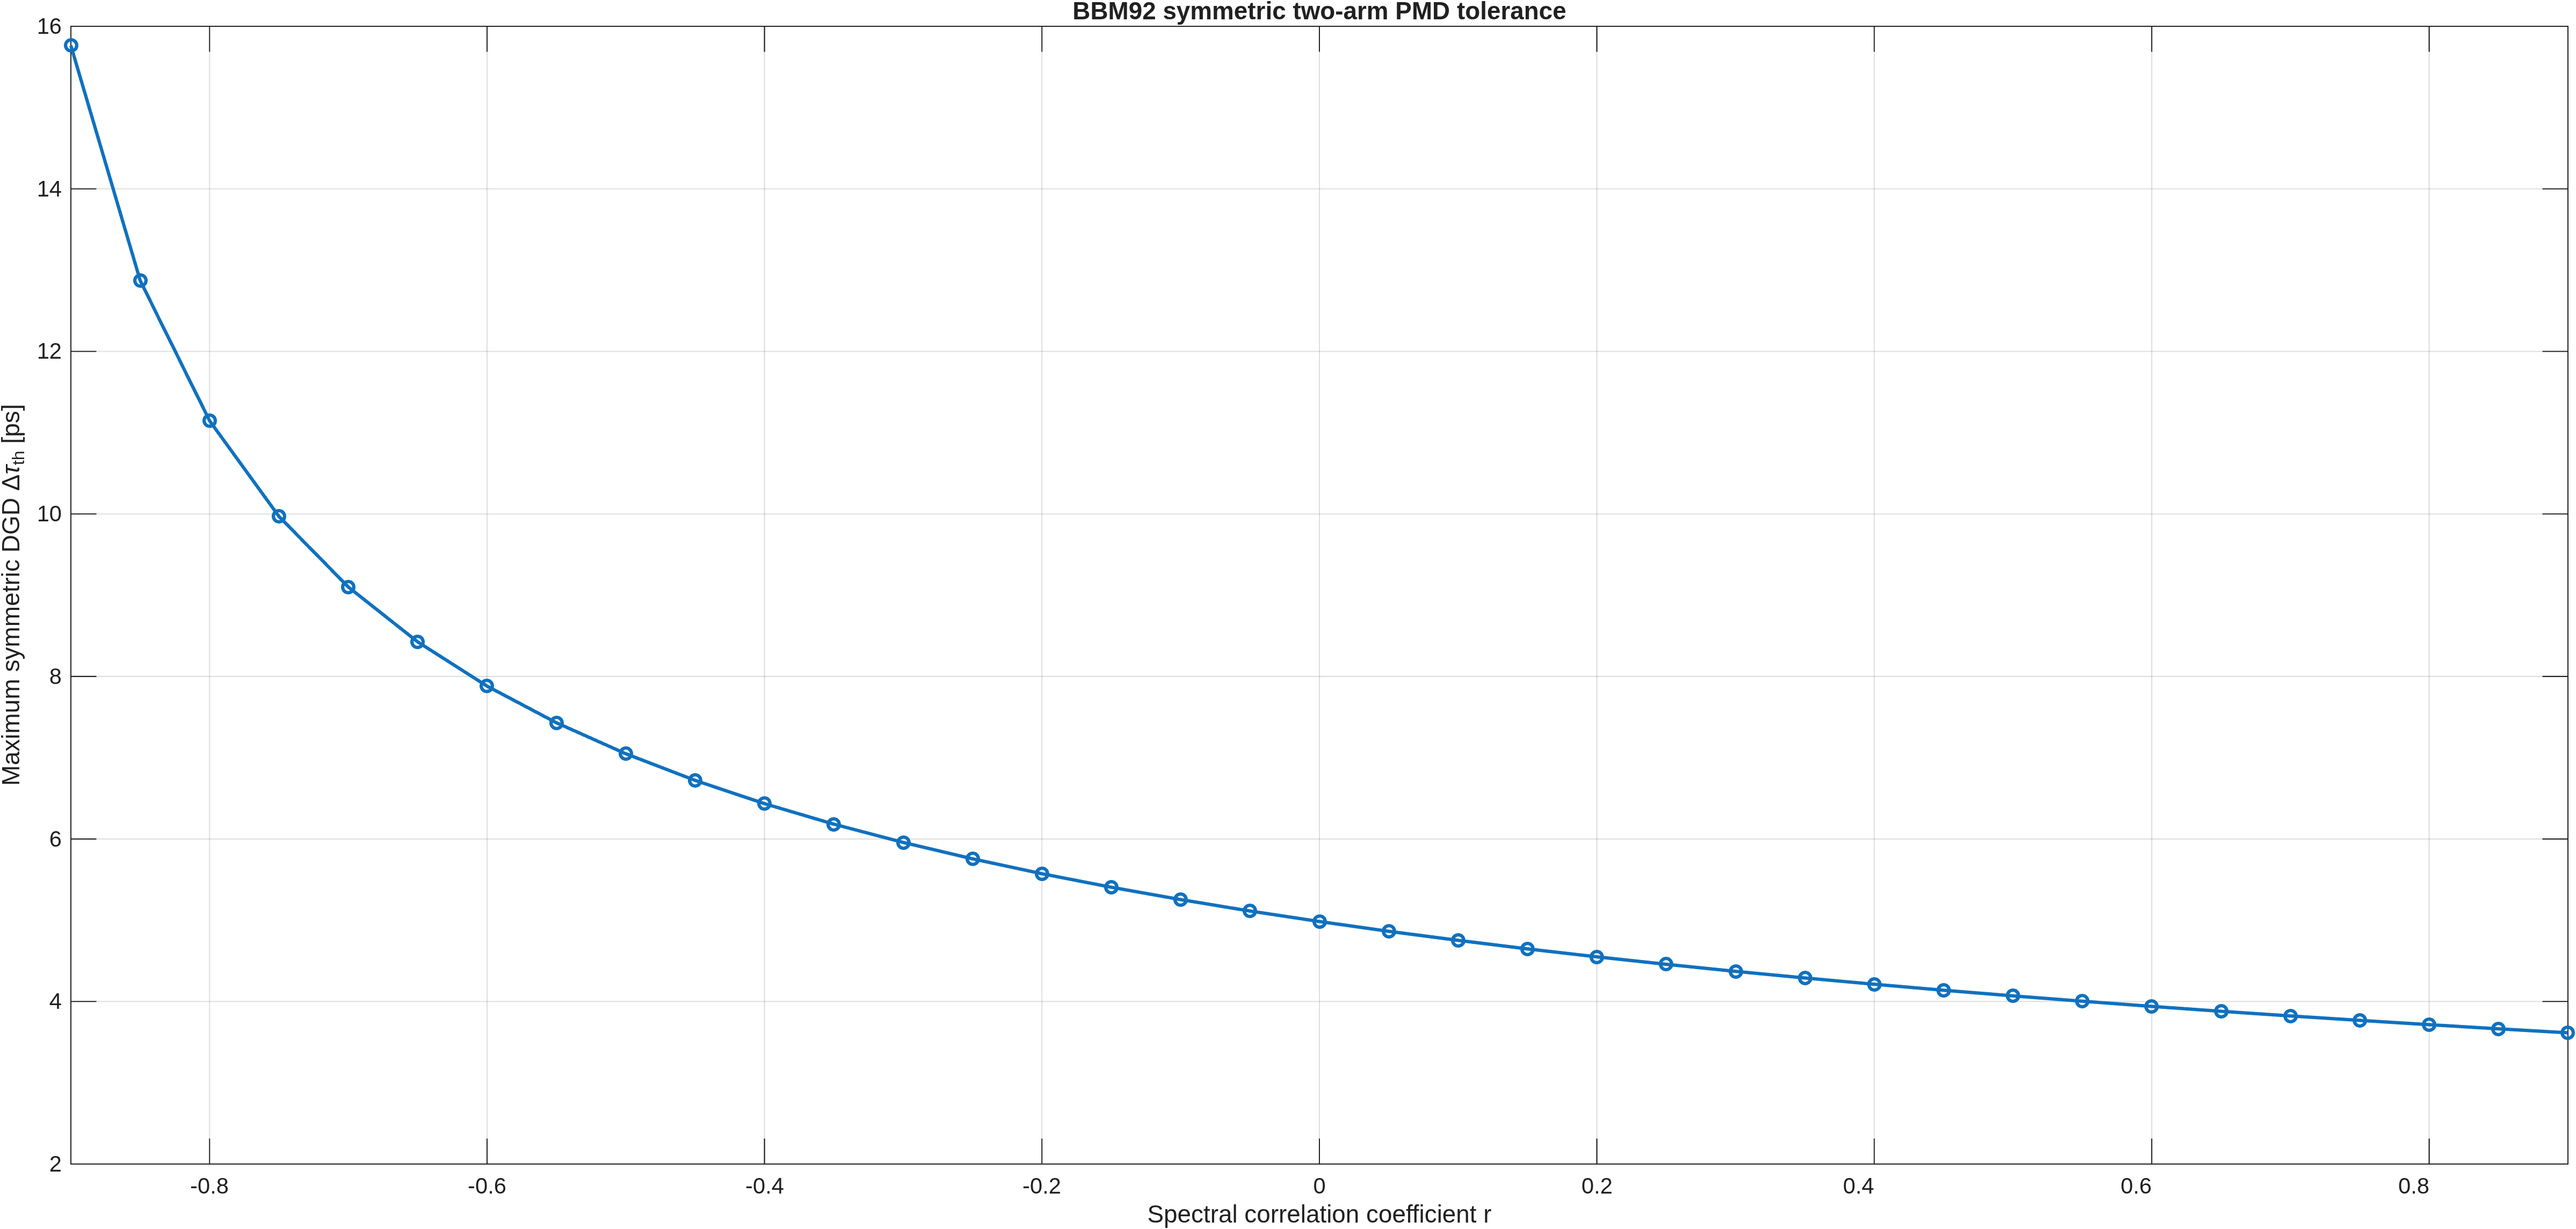
\includegraphics[
        width=0.88\textwidth
    ]{
        figures/experiment_3/spectral_correlation_dgd_boundary.png
    }

    \caption{
        Maximum symmetric differential group delay compatible with the adopted
        BBM92 operating condition as a function of the spectral correlation
        coefficient \(r\), for
        \(\sigma_\omega=1.0\times10^{11}\,\mathrm{rad/s}\).
        Negative spectral correlation substantially increases the tolerable
        symmetric DGD because the anticorrelated frequency offsets partially
        compensate the PMD contributions accumulated in the two aligned fiber
        arms.
    }

    \label{fig:exp3_spectral_correlation_boundary}
\end{figure}

The numerical boundary varies monotonically with the spectral correlation
coefficient. For the three representative conditions, the extracted threshold
DGDs are

\begin{equation}
\begin{aligned}
r=-0.9:
\qquad
\Delta\tau_{\mathrm{th}}
&=
15.763~\mathrm{ps},
\\
r=0:
\qquad
\Delta\tau_{\mathrm{th}}
&=
4.984~\mathrm{ps},
\\
r=+0.9:
\qquad
\Delta\tau_{\mathrm{th}}
&=
3.615~\mathrm{ps}.
\end{aligned}
\label{eq:exp3_symmetric_dgd_results}
\end{equation}

For the fixed source bandwidth considered here, the corresponding normalized
parameters

\begin{equation}
\chi_{\mathrm{th}}
=
\sigma_\omega
\Delta\tau_{\mathrm{th}}
\end{equation}

are

\begin{equation}
\chi_{\mathrm{th}}
=
1.5763,
\qquad
0.4984,
\qquad
0.3615,
\end{equation}

for \(r=-0.9\), \(r=0\), and \(r=+0.9\), respectively.

Moving from strong positive spectral correlation to strong spectral
anticorrelation therefore increases the maximum tolerable symmetric DGD from

\begin{equation}
3.615~\mathrm{ps}
\quad\text{to}\quad
15.763~\mathrm{ps},
\end{equation}

corresponding to an increase by more than a factor of four.

This improvement is obtained without changing either the marginal source
bandwidth or the individual PMD model of the two fibers. It originates entirely
from the different joint spectral statistics of the two photons and their
interaction with the frequency-dependent transformations accumulated in the two
arms.


%--------------------------------------------------------
% Operational Interpretation
%--------------------------------------------------------

\subsection{Operational Interpretation}

The concurrence evaluated at the numerically extracted BBM92 boundary is

\begin{equation}
C_{\mathrm{th}}
\simeq
0.7800
\end{equation}

for all three representative spectral-correlation conditions.

This value is not imposed as an entanglement threshold. The operating boundary
is determined exclusively from

\begin{equation}
Q_{\mathrm{worst}}
=
0.11,
\end{equation}

and the concurrence is evaluated only after the corresponding physical
configuration has been identified. The approximately constant value
\(C\simeq0.78\) is therefore a property of the restricted aligned-axis Gaussian
state family considered here and must not be interpreted as a universal
concurrence requirement for BBM92 operation.

The main result of the experiment is instead that two-arm PMD cannot generally
be characterized by the individual DGDs alone. The same pair of fiber
parameters can produce substantially different polarization degradation
depending on the spectral correlation of the entangled-photon source.

The physical-to-operational mapping investigated in this experiment can
therefore be summarized as

\begin{equation}
\boxed{
\left(
\Delta\tau_A,
\Delta\tau_B,
r
\right)
\longrightarrow
\rho_{\mathrm{pol}}
\longrightarrow
Q_{\mathrm{worst}}
\longrightarrow
\mathcal{R}_{\mathrm{BBM92}}.
}
\label{eq:exp3_final_parameter_mapping}
\end{equation}

Spectral correlation thus becomes an additional source parameter controlling the
robustness of the distributed polarization state against two-arm PMD. In the
specific aligned configuration considered here, strong spectral anticorrelation
can substantially enlarge the BBM92 operating region when the differential group
delays of the two arms are appropriately matched.

%========================================================
% SECTION 3.5 — Experiment 4
%========================================================

\section{Compensation Robustness and Operational Tolerances}
\label{sec:compensation_robustness_operational_tolerances}

The previous experiments characterize the BBM92 operating region under idealized
and controlled PMD configurations. In a practical compensated link, however, the
parameters of the compensating transformation cannot in general be expected to
match the propagation channel exactly.

This experiment will therefore investigate the robustness of the BBM92 operating
region against imperfect PMD compensation. In particular, the analysis will
consider errors in the compensation DGD and misalignment between the relevant
polarization axes. The objective will be to translate these imperfections into
operational tolerances by determining the combinations of compensation errors
for which

\begin{equation}
Q_{\mathrm{worst}}
<
Q_{\mathrm{th}}.
\end{equation}

The resulting maps will provide a direct measure of how accurately the
compensation parameters must reproduce the fiber transformation in order to
maintain the link inside the adopted BBM92 operating region.

% \input{chapters/numerical_simulations/03_4_compensation_robustness_operational_tolerances}


%========================================================
% SECTION 3.6 — Experiment 5
%========================================================

\section{Dependence of the Operating Region on the Fiber Model}
\label{sec:operating_region_model_comparison}

The effective polarization channels introduced in
Chapter~\ref{ch:02_fiber_channel_modeling} provide compact descriptions of
dephasing and depolarization, while the PMD model explicitly includes the
frequency dependence of birefringent propagation and the subsequent spectral
trace.

This experiment will compare the BBM92 operating regions predicted by these
different levels of description. The objective will not be to require the
effective and frequency-dependent models to be physically identical, but rather
to determine under which conditions a reduced polarization-only model provides
an adequate approximation of the operational degradation predicted by the more
detailed PMD description.

The comparison will therefore focus on the displacement of the
\(Q_{\mathrm{worst}}=Q_{\mathrm{th}}\) boundary and will identify parameter
regimes in which the simplified description reproduces the relevant BBM92
operating region, as well as regimes in which the explicit spectral dependence
of the fiber can no longer be neglected.

% \input{chapters/numerical_simulations/03_5_operating_region_model_comparison}


%========================================================
% SECTION 3.7 — Experiment 6
%========================================================

\section{Combined BBM92 Fiber Operating Maps}
\label{sec:combined_bbm92_fiber_operating_maps}

The final numerical experiment will combine the principal physical dependencies
identified throughout the preceding analyses into a unified operational
description of the optical link.

Rather than isolating one propagation mechanism at a time, selected source,
fiber, and compensation parameters will be varied jointly in order to construct
BBM92 operating maps representative of the complete modeling framework developed
in this thesis. The objective will be to identify the regions of the resulting
multidimensional parameter space satisfying

\begin{equation}
\boldsymbol{\xi}
\in
\mathcal{R}_{\mathrm{BBM92}},
\end{equation}

and to determine which physical parameters most strongly constrain the boundary
of this region.

This final analysis will therefore synthesize the results of the preceding
experiments into a set of source--fiber operating conditions, providing the
numerical connection between the physical parameters of the modeled optical link
and its predicted suitability for polarization-entanglement distribution under
the adopted BBM92 criterion.

% \input{chapters/numerical_simulations/03_6_combined_bbm92_fiber_operating_maps}